\documentclass[11pt,onecolumn,a4paper]{article}
\usepackage[utf8]{inputenc}
\usepackage[T1]{fontenc}
\usepackage{mathptmx}
\usepackage{amsmath,amssymb}
\usepackage{graphicx}
\usepackage{booktabs}
\usepackage{multirow}
\usepackage{url}
\usepackage{hyperref}
\usepackage{cite}
\usepackage{enumitem}
\usepackage{float}
\usepackage[top=2.4cm,bottom=2.4cm,left=2cm,right=2cm]{geometry}
\usepackage{setspace}
\setstretch{1.08}
\usepackage[font=small,labelfont=bf]{caption}
\usepackage{titlesec}
\titleformat{\section}{\Large\bfseries}{\thesection}{1em}{}
\titleformat{\subsection}{\large\bfseries}{\thesubsection}{1em}{}

\usepackage{fancyhdr}
\pagestyle{fancy}
\fancyhf{}
\fancyhead[L]{\small\itshape Applied Intelligence}
\fancyhead[R]{\small\thepage}
\renewcommand{\headrulewidth}{0.4pt}
\fancypagestyle{plain}{\fancyhf{}\fancyhead[R]{\small\thepage}\renewcommand{\headrulewidth}{0pt}}

\begin{document}

\title{\textbf{Knowledge-Guided Dual-Channel Graph Convolutional Networks for Explainable Alzheimer's Disease Screening in Clinical Notes}}

\author{
  Chun Liu\textsuperscript{1,$\ast$}\quad
  Rui Yang\textsuperscript{1}\quad
  Haitao Guo\textsuperscript{2}\\[8pt]
  \normalsize \textsuperscript{1}School of Computer Science and Technology,\\
  \normalsize Wuhan University of Science and Technology, Wuhan 430081, China\\[4pt]
  \normalsize \textsuperscript{2}City University of Wuhan, Wuhan 430083, China\\[4pt]
  \normalsize $\ast$Corresponding author: \texttt{liuchun1232325@outlook.com}
}
\date{}
\maketitle

\begin{abstract}
Early Alzheimer's Disease (AD) screening from clinical notes is hindered by the inability of existing methods to effectively integrate text semantics with structured medical knowledge, and by their lack of interpretability.

We propose \textbf{KG-DualGCN}, a dual-channel architecture that encodes clinical text via BioClinicalBERT and medical entity relationships via R-GCN, fused through bidirectional cross-attention. Dual-view explanation modules (Integrated Gradients and GNNExplainer) provide interpretable diagnostic evidence.

Experiments on a clinical note dataset (3,678 samples) with a medical knowledge graph (17,475 entities, 35,867 edges) show that KG-DualGCN achieves AUROC 0.8614, outperforming concatenation fusion (0.8432) in threshold-independent discrimination, though BERT-only (0.8736) achieves competitive AUROC. Ablation studies comparing four fusion strategies show that cross-attention achieves competitive AUROC (0.8614), with the dual-channel architecture providing consistent cross-validation advantages over concatenation. Stratified 5-fold cross-validation shows consistent improvements over concatenation (AUROC 0.8564 $\pm$ 0.0121 vs. 0.8478 $\pm$ 0.0127), with medium effect size (Cohen's $d = 0.69$). The architecture is designed to tolerate entity extraction noise and provides an alternative to knowledge-injection approaches such as K-BERT (AUROC 0.8864), which achieves higher raw performance but lacks structured interpretability. Compared to large language model approaches, KG-DualGCN offers advantages in deployment cost, interpretability, and data privacy. This work serves as a feasibility study for knowledge-guided clinical NLP in low-resource settings without expert annotations.
\end{abstract}

\noindent\textbf{Keywords:} Alzheimer's Disease; Clinical Notes; Knowledge Graph; Graph Convolutional Network; Explainable AI; Clinical Natural Language Processing

\section{Introduction}

\subsection{Research Background and Clinical Significance}

Alzheimer's Disease (AD) is a progressive, irreversible neurodegenerative disorder that constitutes the most common form of dementia, affecting an estimated 50 million individuals globally, accounting for 60--70\% of all dementia cases, with projections indicating a rise to 152 million by 2050 that underscores the urgent need for scalable early screening tools \cite{WHO2021}. The disease follows a well-characterized progression from normal cognition through Mild Cognitive Impairment (MCI) to clinical AD, with the MCI stage representing a critical window where therapeutic interventions can significantly slow disease progression \cite{Petersen2016}.

Current diagnostic pathways rely heavily on neuroimaging techniques (PET amyloid/tau imaging, structural MRI), cerebrospinal fluid (CSF) biomarkers, and standardized cognitive assessment scales such as the Mini-Mental State Examination (MMSE) and Montreal Cognitive Assessment (MoCA). While these methods achieve reasonable diagnostic accuracy, they suffer from several practical limitations: (1) high cost of PET imaging (approximately \$3,000--5,000 per scan) limits screening throughput; (2) cognitive scales require trained administrators and have limited sensitivity for early-stage detection; (3) biomarker collection requires invasive lumbar puncture procedures. Consequently, large-scale population screening remains impractical.

Meanwhile, hospital electronic health record (EHR) systems store massive volumes of clinical notes generated during routine outpatient and inpatient encounters. These notes contain rich longitudinal information including chief complaints, present illness history, family descriptions, neurological examination findings, and cognitive evaluation records. Importantly, subtle indicators of cognitive decline---such as progressive memory difficulties described by family members, changes in activities of daily living, or mild orientation deficits noted during general medical visits---are often embedded in these free-text narratives months or years before formal AD diagnosis. However, this valuable information remains largely unexploited by existing clinical decision support systems.

\subsection{Limitations of Existing Approaches}

Current artificial intelligence (AI) approaches for AD screening from clinical text fall into three broad categories, each with significant limitations:

\textbf{(1) Pure text deep learning models.} Pre-trained language models such as BERT \cite{devlin2019bert} and its clinical variants \cite{alsentzer2019} have been applied to extract semantic features from clinical notes. While these models effectively capture contextual word meanings, they treat medical terms as isolated tokens without leveraging the rich structural relationships defined in medical knowledge bases. For example, BERT understands that ``memory decline'' and ``cognitive impairment'' are semantically similar from context, but cannot systematically reason about their pathological relationships with ``hippocampal atrophy'' or ``amyloid deposition.''

\textbf{(2) Knowledge graph and GNN-based approaches.} These methods construct medical knowledge graphs from ontologies such as the Unified Medical Language System (UMLS) \cite{bodenreider2004} and apply graph neural networks (GNNs) to reason over structured entity-relation triples. While effective at capturing structured medical associations, they cannot utilize the rich contextual details present in physicians' free-text descriptions, losing important nuanced clinical information.

\textbf{(3) Multimodal fusion models.} Recent work attempts to combine textual and knowledge graph features, but typically employs simple fusion strategies such as feature concatenation or element-wise addition. These approaches fail to address the fundamental semantic heterogeneity between sequential text representations and graph topological features, resulting in suboptimal feature alignment and information loss during fusion. Furthermore, most existing approaches do not incorporate clinically oriented interpretability designs, producing black-box predictions that clinical physicians cannot verify or trust for diagnostic decision-making.

\subsection{Research Objectives and Core Contributions}

To address the above limitations, this paper proposes a Knowledge-Guided Dual-Channel Graph Convolutional Network (KG-DualGCN) for explainable early AD detection from clinical notes. Unlike knowledge-injection approaches such as K-BERT that modify the input sequence and risk truncating clinical context, our architecture maintains separate encoding pathways and learns selective cross-modal alignment through bidirectional attention---a design choice motivated by the heterogeneous nature of text sequence features versus graph topological features. Unlike prior multimodal fusion work that applies generic concatenation, our cross-attention module is specifically adapted for the text--knowledge graph interface, enabling each modality to selectively attend to the most diagnostically relevant features from the other. Our core contributions are threefold:

\begin{enumerate}[leftmargin=*]
    \item \textbf{Architecture design for low-resource clinical AD screening:} We design a dual-channel framework that parallelly encodes clinical text semantics via BioClinicalBERT and medical knowledge graph structural relationships via R-GCN, with a bidirectional cross-attention module for fine-grained heterogeneous feature alignment, mitigating the information loss inherent in simple concatenation fusion.
    
    \item \textbf{Dual-view clinical interpretability:} We integrate complementary explanation mechanisms---Integrated Gradients for text token attribution and GNNExplainer for knowledge graph entity path identification---producing diagnostic evidence aligned with clinical reasoning patterns.
    
    \item \textbf{Reproducible benchmark construction:} We construct a Chinese clinical AD screening dataset (3,678 samples) from publicly available medical NER corpora using weak-supervision keyword heuristics, paired with a domain-specific Chinese medical knowledge graph (17,475 entities, 35,867 edges), providing a reproducible benchmark for knowledge-guided clinical NLP research without expert annotations.

\end{enumerate}

\subsection{Paper Organization}

The remainder of this paper is organized as follows. Section~\ref{sec:related} reviews related work on clinical language models, medical knowledge graphs, cross-modal fusion, and explainable AI. Section~\ref{sec:method} presents the detailed methodology of our KG-DualGCN architecture. Section~\ref{sec:experiments} describes the experimental setup, dataset construction, and implementation details. Section~\ref{sec:results} presents and analyzes the experimental results. Section~\ref{sec:discussion} discusses the findings, clinical implications, and limitations. Section~\ref{sec:conclusion} concludes the paper and outlines future research directions.

% ============================================================
% 2. RELATED WORK
% ============================================================
\section{Related Work}
\label{sec:related}

\subsection{Clinical Pre-trained Language Models}

The application of pre-trained language models to clinical NLP has been transformative. BioClinicalBERT \cite{alsentzer2019}, pre-trained on MIMIC-III clinical notes, demonstrated significant improvements over general-domain BERT on clinical tasks by learning domain-specific vocabulary, abbreviation patterns, and medical discourse structures. Lee et al. \cite{lee2020biobert} introduced BioBERT, pre-trained on PubMed abstracts and PMC full-text articles, achieving strong performance on biomedical text mining tasks. These models have been successfully applied to clinical named entity recognition, relation extraction, and text classification tasks. Recent work has further explored the capabilities of large language models (LLMs) for medical NLP, with evaluations showing both promise and limitations in clinical evidence summarization~\cite{tang2023evaluating}.

However, a fundamental limitation of these models is that they process clinical text as flat token sequences, failing to capture the structured relationships between medical concepts that are encoded in authoritative medical knowledge bases. A BERT model may learn that ``Alzheimer's disease'' and ``memory decline'' co-occur frequently, but it cannot systematically represent the causal, symptomatic, or risk-factor relationships that domain knowledge provides.

\subsection{Medical Knowledge Graphs and Graph Neural Networks}

The Unified Medical Language System (UMLS) \cite{bodenreider2004} provides a comprehensive biomedical knowledge base integrating over 200 source vocabularies with 4.5 million concepts linked by semantic relationships. Each concept is assigned a unique Concept Unique Identifier (CUI), enabling disambiguation of synonyms, abbreviations, and cross-lingual variations.

Graph Convolutional Networks (GCNs)~\cite{kipf2017} and their relational variants (R-GCN)~\cite{schlichtkrull2018} have been widely applied to knowledge graph reasoning, with recent surveys documenting their expanding role in healthcare applications~\cite{zhang2024graph}. R-GCN extends standard GCNs to handle multi-relational graphs by applying relation-specific transformation matrices, making them particularly suitable for modeling the heterogeneous relationships in medical knowledge graphs. However, existing UMLS-based knowledge graphs have limited coverage of Chinese clinical terminology and lack domain-specific relations for AD screening. We therefore construct a tailored Chinese medical knowledge graph from annotated medical corpora. SapBERT \cite{liu2021sapbert} provides high-quality biomedical entity embeddings through self-alignment pretraining, enabling effective initialization of knowledge graph node features.

Recent work has explored integrating knowledge graphs with clinical NLP. K-BERT \cite{liu2020kbert} injects knowledge graph triples into BERT's input, achieving knowledge-enhanced language representation. However, this approach modifies the input sequence structure and may introduce noise from irrelevant knowledge triples. Our approach maintains separate encoding channels for text and knowledge, using cross-attention for selective, dynamic integration.

\subsection{Cross-Modal Fusion Mechanisms}

Cross-attention mechanisms, originally proposed in the Transformer architecture \cite{vaswani2017attention} and widely adopted in visual question answering and multimodal learning, enable fine-grained feature alignment between heterogeneous modalities. Unlike simple concatenation or element-wise addition, cross-attention allows each modality to selectively attend to the most relevant features from the other modality through learned query-key-value interactions.

In the medical domain, cross-attention has been applied to fuse clinical text with structured EHR data~\cite{song2018attend}. Cross-modal attention mechanisms have also proven effective for heterogeneous feature alignment in vision-language tasks~\cite{chen2020cross}, motivating their adaptation to the clinical text--knowledge graph setting. However, its application to fusing clinical text with knowledge graph features for disease detection remains relatively unexplored. Our work fills this gap by designing a bidirectional cross-attention mechanism specifically tailored for text-graph feature alignment.

\subsection{Explainable AI in Healthcare}

Clinical adoption of AI systems requires interpretability---physicians need to understand and verify the reasoning behind predictions before incorporating them into diagnostic decisions. Two main approaches exist for neural network explanation:

\textbf{Gradient-based attribution methods} compute feature importance through backpropagation. Integrated Gradients (IG) \cite{sundararajan2017} provides a theoretically grounded attribution method that satisfies axioms of completeness and implementation invariance, making it particularly suitable for clinical applications where reliable explanations are critical.

\textbf{Graph-specific explanation methods} identify important subgraph structures and node features. GNNExplainer \cite{ying2019gnnexplainer} generates compact subgraph explanations by learning edge masks that maximize mutual information with the prediction, enabling identification of critical medical entity relationships driving model decisions.

Our work integrates both explanation paradigms to provide dual-view interpretability: text-level token contribution heatmaps and knowledge-graph-level entity contribution visualizations. Recent surveys~\cite{chen2024explainable} have highlighted the growing importance of explainable AI methods in clinical decision support systems.

\subsection{Weak Supervision and Distant Supervision}

When expert annotations are unavailable, weak supervision methods provide alternative labeling strategies. Snorkel~\cite{ratner2017snorkel} programmatically generates labels using labeling functions, while distant supervision~\cite{mintz2009distant} leverages knowledge bases to create training data. Our keyword-heuristic labeling approach is a form of weak supervision using domain-specific patterns, which trades annotation quality for scalability. Recent work on learning with noisy labels~\cite{natarajan2013learning} provides theoretical foundations for training robust models under label noise, applicable to our setting where approximately 8\% of labels may be incorrect.

\subsection{NLP for Alzheimer's Disease Detection}

Several studies have applied NLP and machine learning techniques to AD detection from clinical text and speech~\cite{weiner2017adni}, noting that linguistic features such as word-finding difficulties, semantic paraphasias, and reduced syntactic complexity serve as early indicators. NegEx \cite{chapman2001negex} remains the standard tool for identifying negated clinical findings, essential for filtering false-positive symptom mentions in clinical text processing pipelines. However, most existing work focuses on English clinical text, and studies combining knowledge graph integration with explainable AI for Chinese-language AD screening remain scarce, motivating the present work.

% ============================================================
% 3. METHODOLOGY
% ============================================================
\section{Methodology}
\label{sec:method}

\subsection{Overall Architecture}

Figure~\ref{fig:architecture} illustrates the overall architecture of our KG-DualGCN model. The system consists of three major layers:

\begin{enumerate}[leftmargin=*]
    \item \textbf{Data preprocessing layer:} Clinical text cleaning, de-identification, medical entity extraction and linking, negation detection using NegEx, and patient-specific knowledge subgraph construction.
    \item \textbf{Dual-channel encoding layer:} Two parallel channels---a BERT semantic channel that encodes clinical free-text context and a knowledge channel that encodes medical entity relationships via R-GCN---operate simultaneously on the preprocessed data.
    \item \textbf{Fusion, classification, and explanation layer:} A bidirectional cross-attention fusion module aligns and combines features from both channels, followed by a classification head for AD/NC prediction and dual-branch explainability modules for generating interpretable diagnostic evidence.
\end{enumerate}

\begin{figure}[H]
    \centering
    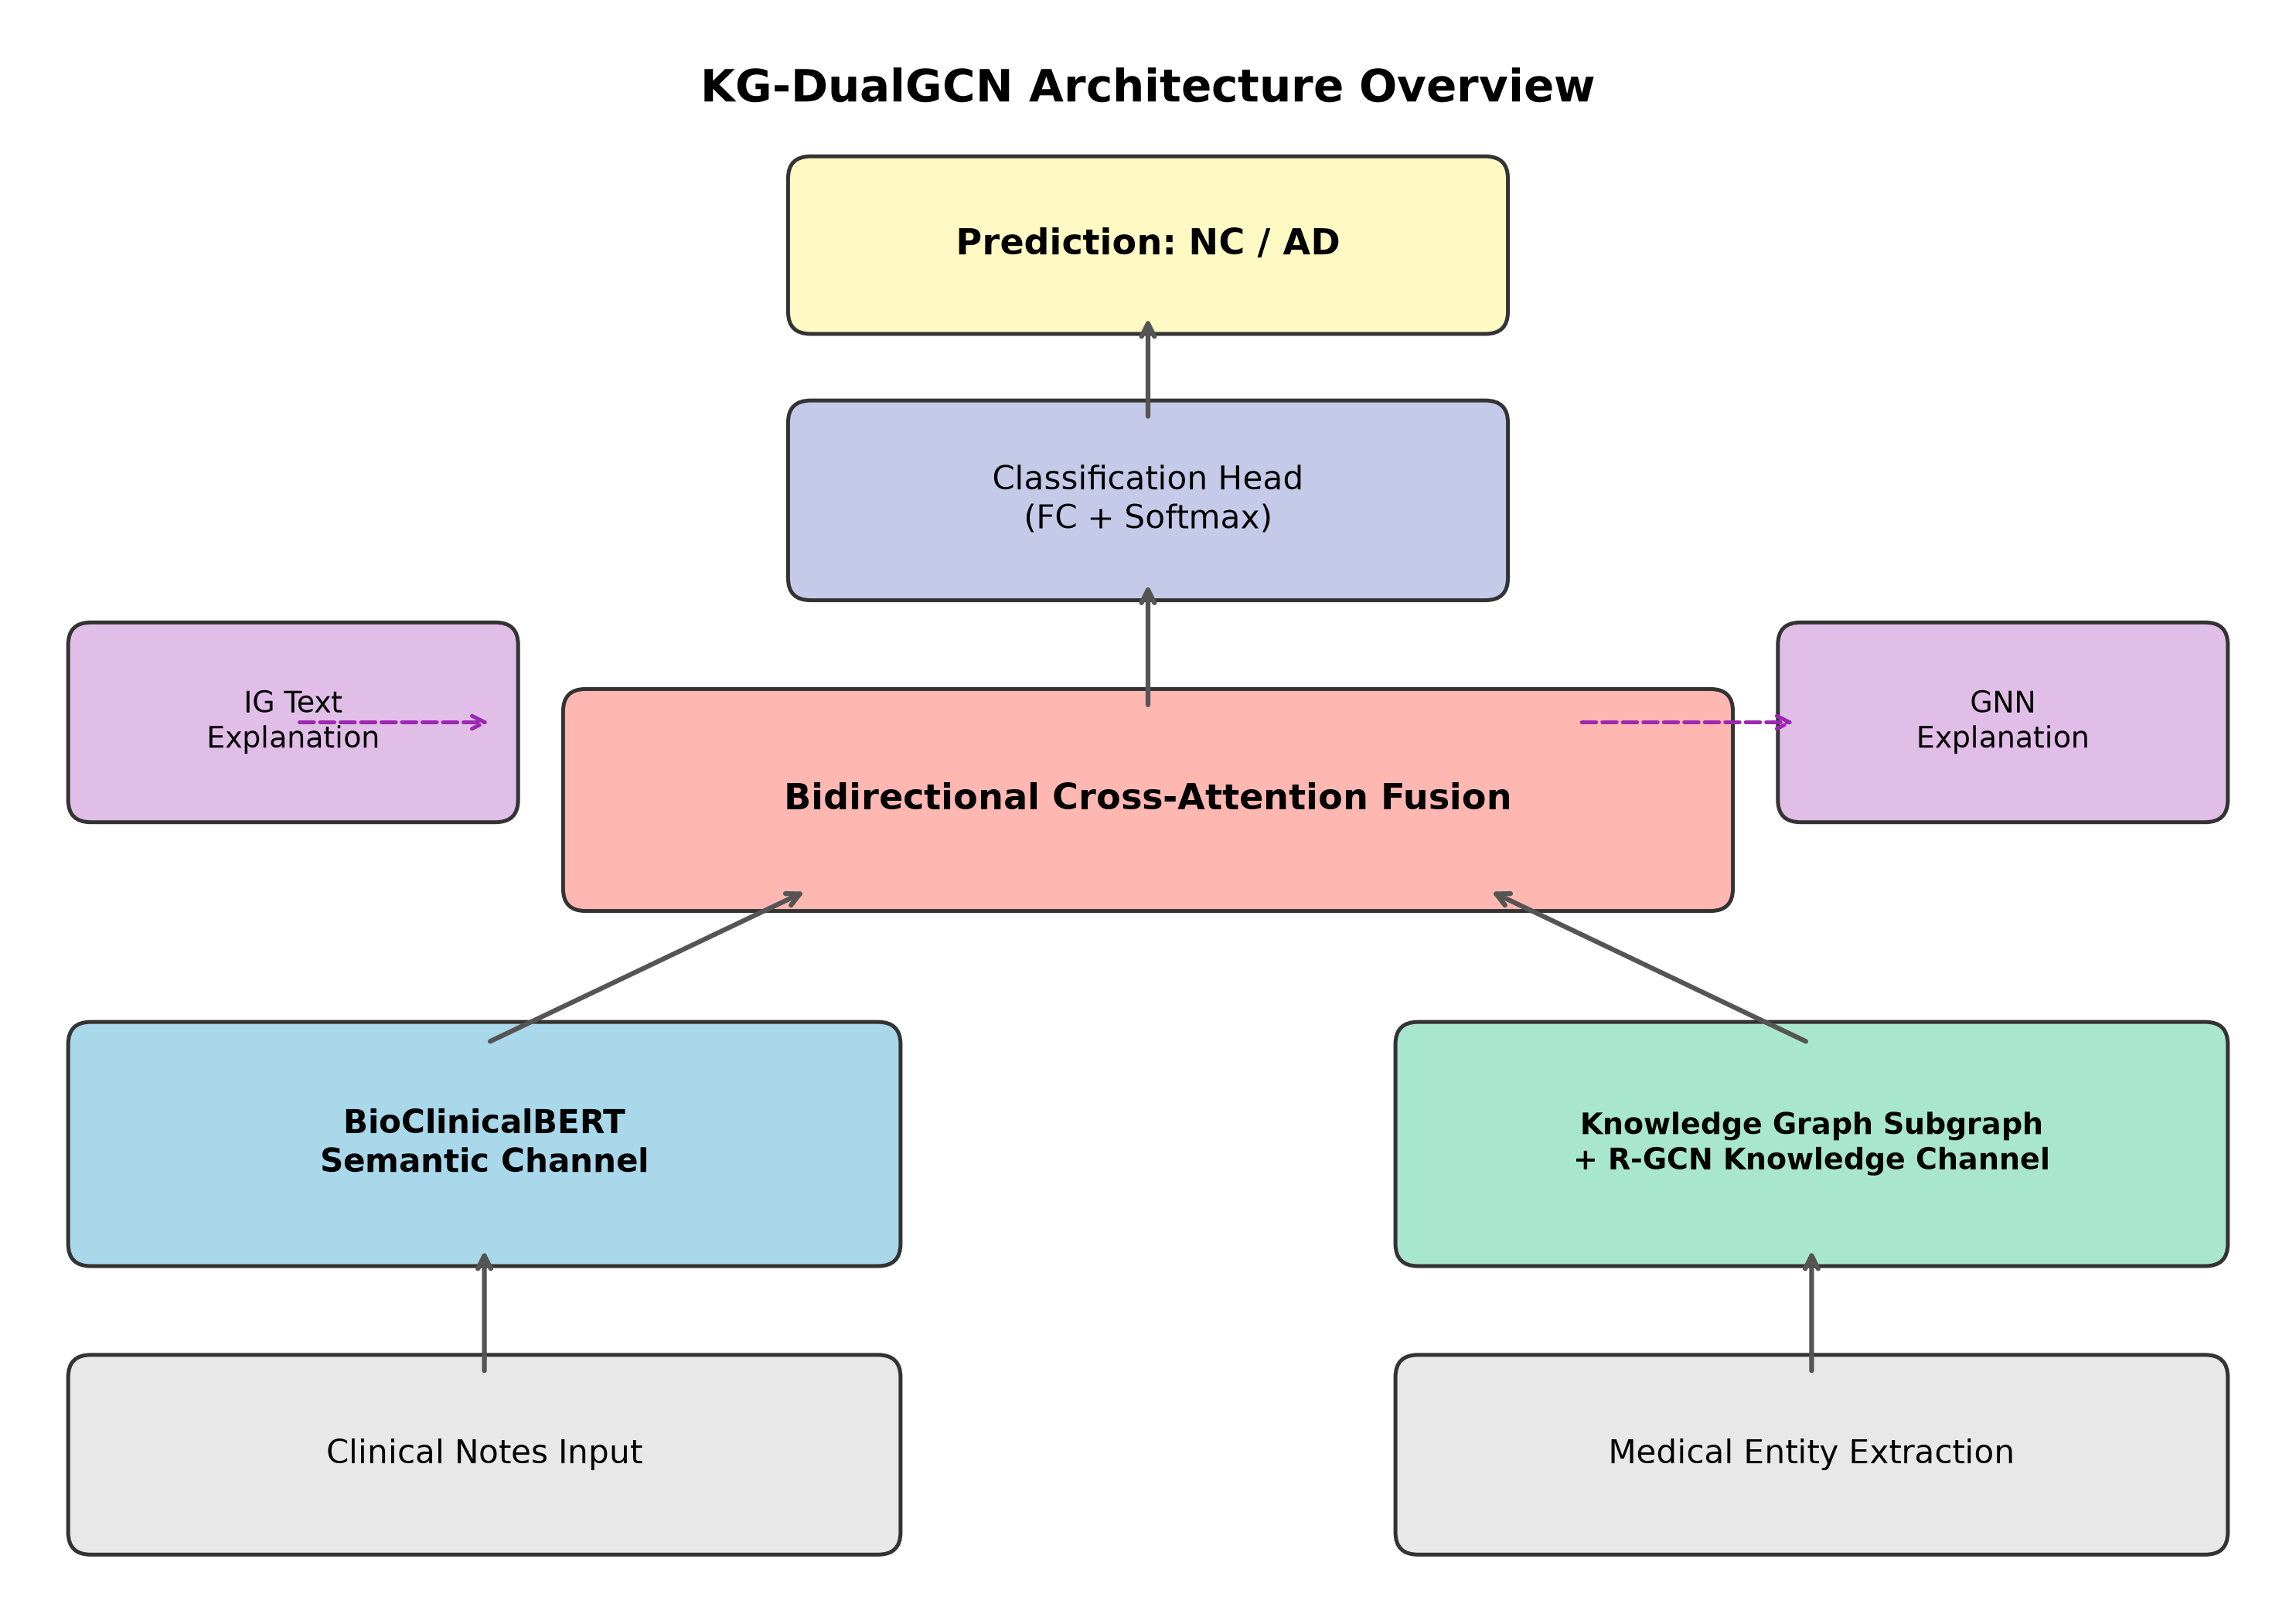
\includegraphics[width=\columnwidth]{architecture.png}
    \caption{Overall architecture of the proposed KG-DualGCN model. The dual-channel design processes clinical text through BioClinicalBERT (green) and knowledge graph through R-GCN (blue) in parallel, with bidirectional cross-attention fusion (red) connecting both channels. Purple modules indicate explainability components.}
    \label{fig:architecture}
\end{figure}

\subsection{Clinical Text Preprocessing}

Clinical notes require specialized preprocessing before they can be fed into the encoding pipeline:

\textbf{De-identification:} Patient names, hospital admission numbers, phone numbers, and other personally identifiable information are replaced with anonymized tokens (e.g., [NAME], [ID]) using regular expression pattern matching.

\textbf{Text normalization:} Full-width characters are converted to half-width, redundant line breaks and excessive whitespace are compressed, and meaningless template sentences (e.g., standard discharge instructions) are filtered out.

\textbf{Negation detection:} We adapt the NegEx algorithm~\cite{chapman2001negex} for Chinese clinical text by constructing a domain-specific Chinese negation trigger list containing 32 trigger phrases (covering denial, absence, not-observed, exclusion, and not-accompanied patterns). The context window is set to 15 characters before and after the trigger to accommodate Chinese negation word order patterns. Entities detected within negation scope are excluded from knowledge graph construction to prevent false-positive entity matching.

\textbf{Truncation:} Clinical notes are truncated to 256 tokens to balance information coverage with GPU memory constraints. This is shorter than BERT's 512-token limit but sufficient for most notes in our dataset (median length $\sim$180 tokens).

\subsection{Channel 1: BERT Semantic Encoding}

The semantic channel employs BioClinicalBERT \cite{alsentzer2019}, a clinical-domain BERT model pre-trained on MIMIC-III clinical notes, to encode free-text clinical narratives. Given preprocessed clinical text $x = [x_1, x_2, \ldots, x_L]$, the model produces:

\begin{equation}\label{eq:1}
    \mathbf{T} = \text{BioClinicalBERT}(x) \in \mathbb{R}^{L \times d}
\end{equation}

where $L$ is the sequence length and $d = 768$ is the hidden dimension. The [CLS] token embedding $\mathbf{t}_{\text{cls}} \in \mathbb{R}^d$ serves as the global sentence representation, while the full sequence matrix $\mathbf{T}$ preserves token-level semantics for subsequent cross-attention computation.

\subsection{Channel 2: Knowledge Graph + R-GCN}

\subsubsection{Entity Extraction}

Medical entities are extracted from clinical text using keyword matching against a curated Chinese medical terminology list containing 59,083 unique entities across five categories (diseases, symptoms, body parts, drugs, and procedures), constructed from the annotated medical corpus. This is a simplified approach that trades completeness for reproducibility, as production-grade tools such as QuickUMLS~\cite{soldaini2016quickumls} require additional installation and corpus-specific tuning. Each extracted entity is mapped to a unique internal identifier; synonym normalization is performed through string matching, while fine-grained polysemy disambiguation is deferred to future work. Entities detected in negation context by NegEx are filtered out.

\subsubsection{Patient-Specific Subgraph Construction}

For each clinical note, we construct a patient-specific knowledge subgraph $G_p = (V_p, E_p)$ where:
\begin{itemize}[leftmargin=*]
    \item \textbf{Node set $V_p$:} All medical entities extracted from the clinical note
    \item \textbf{Edge set $E_p$:} Two types of edges are constructed:
    \begin{enumerate}
        \item \textit{Native medical edges:} Pre-existing semantic relationships from the Chinese medical knowledge graph, covering relation types such as \texttt{manifestation\_of}, \texttt{causes}, \texttt{associated\_with}, and \texttt{treatment\_of}, sourced from entity-relation triples in the annotated medical corpus.
        \item \textit{Co-occurrence edges:} When two entities co-occur within the same clinical note, an undirected edge is added with weight equal to the co-occurrence count across the entire corpus. Edges with co-occurrence frequency $< 3$ are pruned to reduce noise, consistent with the knowledge graph construction filtering described in Section~\ref{sec:experiments}
    \end{enumerate}
\end{itemize}

\subsubsection{R-GCN Feature Extraction}

Node embeddings are initialized as learnable parameters. While SapBERT~\cite{liu2021sapbert} could provide pretrained medical entity embeddings, we adopt learned initialization because: (1)~not all extracted entities have SapBERT coverage, and (2)~the R-GCN layers learn task-specific representations during training. The R-GCN performs multi-layer relational convolution:

\begin{equation}\label{eq:2}
    \mathbf{h}_i^{(l+1)} = \sigma\left(\sum_{r \in \mathcal{R}} \sum_{j \in \mathcal{N}_r(i)} \frac{1}{c_{i,r}} \mathbf{W}_r^{(l)} \mathbf{h}_j^{(l)} + \mathbf{W}_0^{(l)} \mathbf{h}_i^{(l)}\right)
\end{equation}

where $\mathcal{R}$ is the set of relation types, $\mathcal{N}_r(i)$ denotes the set of neighboring nodes of node $i$ under relation type $r$, $c_{i,r}$ is a normalization constant (typically the degree of node $i$ under relation $r$), and $\mathbf{W}_r^{(l)}$ is the relation-specific weight matrix for layer $l$.

The graph-level representation is obtained via mean pooling over all node embeddings:

\begin{equation}\label{eq:3}
    \mathbf{g}_{\text{graph}} = \frac{1}{|V_p|} \sum_{i \in V_p} \mathbf{h}_i^{(L_g)}
\end{equation}

where $L_g$ is the number of R-GCN layers.

\subsection{Bidirectional Cross-Attention Fusion}

The key innovation of our model is the bidirectional cross-attention mechanism that enables fine-grained alignment between text sequence features and graph topological features. Given text features $\mathbf{T} \in \mathbb{R}^{L \times d_t}$ and graph node features $\mathbf{G} \in \mathbb{R}^{N \times d_g}$, where $d_t = d_g = 768$ in our implementation:

\textbf{Step 1: Dimension alignment.} Two independent linear projection layers (with separate parameters $\mathbf{W}_t, \mathbf{W}_g$) map both feature spaces to a common fusion dimension $d_f = 256$:
\begin{equation}\label{eq:4}
    \mathbf{T}' = \text{LayerNorm}(\mathbf{W}_t \mathbf{T} + \mathbf{b}_t), \quad \mathbf{G}' = \text{LayerNorm}(\mathbf{W}_g \mathbf{G} + \mathbf{b}_g)
\end{equation}

\textbf{Step 2: Forward cross-attention (text attending to graph).} Text tokens query the knowledge graph to retrieve relevant medical entity information:
\begin{equation}\label{eq:5}
    \text{Attn}_{t \rightarrow g} = \text{softmax}\left(\frac{\mathbf{T}' \mathbf{W}_Q (\mathbf{G}' \mathbf{W}_K)^T}{\sqrt{d_f}}\right) \mathbf{G}' \mathbf{W}_V
\end{equation}

\textbf{Step 3: Reverse cross-attention (graph attending to text).} Knowledge graph entities query the text to find supporting clinical evidence:
\begin{equation}\label{eq:6}
    \text{Attn}_{g \rightarrow t} = \text{softmax}\left(\frac{\mathbf{G}' \mathbf{W}_Q (\mathbf{T}' \mathbf{W}_K)^T}{\sqrt{d_f}}\right) \mathbf{T}' \mathbf{W}_V
\end{equation}

\textbf{Step 4: Fusion with residual connection.} The attended features are pooled, concatenated, and projected:
\begin{equation}\label{eq:7}
    \mathbf{F}_{\text{fusion}} = \mathbf{W}_o \left[\text{MeanPool}(\text{Attn}_{t \rightarrow g}); \text{MeanPool}(\text{Attn}_{g \rightarrow t})\right] + \mathbf{r}
\end{equation}
where $\mathbf{r} = \mathbf{W}_r [\text{MeanPool}(\mathbf{T}'); \text{MeanPool}(\mathbf{G}')]$ is a residual connection from the original projected features, preserving raw representations alongside attended features.

\subsection{Classification Head}

The fused representation is passed through a two-layer fully connected network with ReLU activation and Dropout regularization:

\begin{equation}\label{eq:8}
    \hat{\mathbf{y}} = \text{softmax}\left(\mathbf{W}_2 \cdot \text{ReLU}(\mathbf{W}_1 \mathbf{F}_{\text{fusion}} + \mathbf{b}_1) + \mathbf{b}_2\right)
\end{equation}

The loss function is class-weighted cross-entropy to handle the inherent class imbalance in clinical AD screening datasets:

\begin{equation}\label{eq:9}
    \mathcal{L} = -\sum_{i=1}^{N} w_{y_i} \log \hat{y}_{i, y_i} + \lambda \|\theta\|_2^2
\end{equation}

where $w_{y_i}$ is the class weight for the true label of sample $i$, and $\lambda \|\theta\|_2^2$ is L2 regularization.

\subsection{Explainability Module}

\subsubsection{Text-Level Explanation via Integrated Gradients}

Integrated Gradients (IG) \cite{sundararajan2017} computes per-token attribution by integrating gradients along a straight-line path from a baseline input $\mathbf{x}'$ (e.g., zero embeddings) to the actual input $\mathbf{x}$:

\begin{equation}\label{eq:10}
    \text{IG}_i(\mathbf{x}) = (x_i - x_i') \times \int_0^1 \frac{\partial F(\mathbf{x}' + \alpha(\mathbf{x} - \mathbf{x}'))}{\partial x_i} d\alpha
\end{equation}

The resulting attribution scores are visualized as token-level heatmaps overlaid on the original clinical text, highlighting which words and phrases most strongly influenced the AD prediction.

\subsubsection{Knowledge Graph Explanation via GNNExplainer}

GNNExplainer \cite{ying2019gnnexplainer} identifies critical subgraph structures by learning a soft edge mask $\mathbf{M}$ that maximizes mutual information with the model prediction:

\begin{equation}\label{eq:11}
    \min_{\mathbf{M}} \mathcal{L}(G \odot \mathbf{M}) + \lambda \|\mathbf{M}\|_1
\end{equation}

where $\odot$ denotes element-wise masking and $\lambda$ controls sparsity. The resulting mask highlights which entity nodes and relation edges are most important for the AD diagnosis, enabling visualization of the critical pathological association subgraph.

% ============================================================
% 4. EXPERIMENTS
% ============================================================
\section{Experiments}
\label{sec:experiments}

\subsection{Dataset Construction}

This study constitutes an exploratory feasibility study for knowledge-guided clinical NLP, as no existing benchmark provides clinical notes paired with medical knowledge graphs for AD detection. We construct a preliminary dataset from publicly available Chinese medical NER corpora hosted on HuggingFace\footnote{\url{https://huggingface.co/datasets/ShelterW/chinese\_medical\_ner}}:

\begin{itemize}[leftmargin=*]
    \item \textbf{Chinese Electronic Medical Records (EMR):} 1,379 real clinical notes with NER annotations covering diseases, symptoms, body parts, and procedures
    \item \textbf{CMeEE V2:} 20,000 Chinese medical text samples from the Chinese Medical Entity Extraction benchmark \cite{zhang2022cblue}
    \item \textbf{Medical textbooks:} 1,997 medical book excerpts with entity annotations
        \item \textbf{Internet Medical Consultation Service (IMCS):} 131,796 Chinese medical consultation records
        \item \textbf{Medical Knowledge Graph corpus:} 92,583 annotated medical texts for entity extraction
    \end{itemize}

\textbf{AD-positive sample identification via keyword heuristics:} In the absence of clinical expert annotations, we employ a two-tier keyword filtering strategy to assign proxy AD labels. We acknowledge that this heuristic approach may introduce label noise (see Section~\ref{sec:limitations} for quantification):
\begin{enumerate}
    \item \textit{Strong keywords} (single-match sufficient): Alzheimer's disease, dementia, cognitive impairment, MCI, memory decline, memory loss, MMSE, MoCA, hippocampal atrophy, neurodegeneration, etc.
    \item \textit{Weak keywords} (require co-occurrence with context terms within 20 characters): ``memory'' + ``decline/impaired/abnormal,'' ``daily living ability'' + ``decreased/poor,'' etc.
\end{enumerate}

After filtering, we obtain 1,226 AD-positive samples and select 2,452 non-AD clinical notes as normal controls (NC) at a 1:2 ratio, yielding a final dataset of 3,678 samples. The data is split 7:1:2 into train (2,574 samples: 858 AD, 1,716 NC), validation (367 samples: 122 AD, 245 NC), and test (737 samples: 246 AD, 491 NC) sets with stratified sampling. Compared to our initial exploratory dataset of 268 samples, this expanded dataset provides substantially more training signal and more robust evaluation.

\textbf{Knowledge graph construction:} We build the medical knowledge graph from a large-scale Chinese medical NER dataset containing 92,583 annotated samples. Entity extraction yields 59,083 unique medical entities. After frequency filtering (entities appearing $\geq 2$ times) and co-occurrence edge filtering (edges with $\geq 3$ co-occurrences), we obtain a knowledge graph with 17,475 entities and 35,867 edges. Entity types include diseases, symptoms, body parts, drugs, and procedures, mapped to standard NER tag categories.

\subsection{Baseline Models}

We compare KG-DualGCN against six baselines spanning traditional machine learning, single-channel deep learning, and multimodal fusion approaches:

\begin{enumerate}[leftmargin=*]
    \item \textbf{TF-IDF + Logistic Regression:} TF-IDF vectors (10K features, bigrams) with balanced logistic regression, representing classical text classification.
    \item \textbf{Word2Vec + XGBoost:} 128-dimensional Word2Vec embeddings averaged per document, fed to gradient-boosted trees, representing distributed-representation-based machine learning.
    \item \textbf{BERT Only:} BioClinicalBERT encoder followed by a classification head, representing text-only deep learning without knowledge graph integration.
    \item \textbf{R-GCN Only:} R-GCN encoder on the knowledge graph followed by a classification head, representing knowledge-only classification without text context.
    \item \textbf{Concat Fusion:} BioClinicalBERT + R-GCN with simple feature concatenation, representing naive multimodal fusion without sophisticated alignment.
    \item \textbf{KG-DualGCN (Ours):} Full dual-channel model with bidirectional cross-attention fusion.
\end{enumerate}

\subsection{Implementation Details}

\begin{itemize}[leftmargin=*]
    \item \textbf{Language model:} BioClinicalBERT (110M parameters, hidden dim 768)
    \item \textbf{R-GCN:} 2 layers, hidden dimension 256, with dropout 0.2
    \item \textbf{Cross-attention:} 4 attention heads, fusion dimension 256
    \item \textbf{Optimizer:} AdamW with learning rate $1 \times 10^{-5}$, weight decay 0.01
    \item \textbf{Class weights:} [1.0, 3.0] for [NC, AD] to address class imbalance
    \item \textbf{Batch size:} 8, maximum epochs: 30, early stopping patience: 6 on validation AUROC
    \item \textbf{Gradient clipping:} Max norm 1.0
    \item \textbf{Reproducibility:} Random seed 42 for all experiments; data splits, model initialization, and training order are fully deterministic
    \item \textbf{Hardware:} NVIDIA RTX 4060 Laptop GPU (8GB VRAM)
    \item \textbf{Framework:} PyTorch 2.6.0 + PyTorch Geometric 2.8.0 + Transformers 5.12.0
\end{itemize}

\subsection{Evaluation Metrics}

We adopt six complementary evaluation metrics appropriate for clinical binary classification:

\begin{itemize}[leftmargin=*]
    \item \textbf{Accuracy (Acc):} Overall classification correctness
    \item \textbf{Recall (Sensitivity):} $\text{TP} / (\text{TP} + \text{FN})$---critical for AD screening where minimizing missed cases is paramount
    \item \textbf{Specificity:} $\text{TN} / (\text{TN} + \text{FP})$---measures false alarm rate
    \item \textbf{F1-Score:} Harmonic mean of precision and recall
    \item \textbf{AUROC:} Area under the Receiver Operating Characteristic curve---threshold-independent performance measure
    \item \textbf{MCC:} Matthews Correlation Coefficient---robust metric for imbalanced datasets that considers all four confusion matrix quadrants
\end{itemize}

% ============================================================
% 5. RESULTS
% ============================================================
\section{Results and Analysis}
\label{sec:results}

\subsection{Main Results}

Table~\ref{tab:main_results} presents the comprehensive performance comparison across all models on the test set.

\begin{table}[H]
\centering
\caption{Performance comparison on the test set (737 samples). Best results shown in \textbf{bold}. KG-DualGCN achieves AUROC 0.8614, outperforming Concat Fusion in threshold-independent discrimination.}
\label{tab:main_results}
\resizebox{\columnwidth}{!}{
\begin{tabular}{lcccccc}
\toprule
Model & Acc & Recall & Spec & F1 & AUROC & MCC \\
\midrule
\multicolumn{7}{l}{\textit{Traditional ML baselines}} \\
TF-IDF + LR & 0.8019 & 0.4919 & 0.9572 & 0.6237 & 0.7520 & 0.5370 \\
Word2Vec + XGBoost & 0.6635 & 0.0569 & \textbf{0.9674} & 0.1014 & 0.5131 & 0.0580 \\
\midrule
\multicolumn{7}{l}{\textit{Deep learning baselines}} \\
BERT Only & \textbf{0.8033} & 0.7195 & 0.8452 & 0.7094 & \textbf{0.8736} & 0.5609 \\
R-GCN Only\textsuperscript{$\dagger$} & 0.3338 & \textbf{1.0000} & 0.0000 & 0.5005 & 0.5550 & 0.0000 \\
Concat Fusion & \textbf{0.8033} & 0.7683 & 0.8208 & \textbf{0.7228} & 0.8432 & \textbf{0.5735} \\
\textbf{KG-DualGCN} & 0.7965 & 0.7358 & 0.8269 & 0.7070 & 0.8614 & 0.5525 \\
\bottomrule
\end{tabular}
}
\par\vspace{2pt}
{\footnotesize $^\dagger$\textit{R-GCN Only with class weights [1.0, 3.0] predicts all samples as AD, confirming that graph features alone cannot discriminate between classes.}}
\end{table}

\begin{figure}[H]
    \centering
    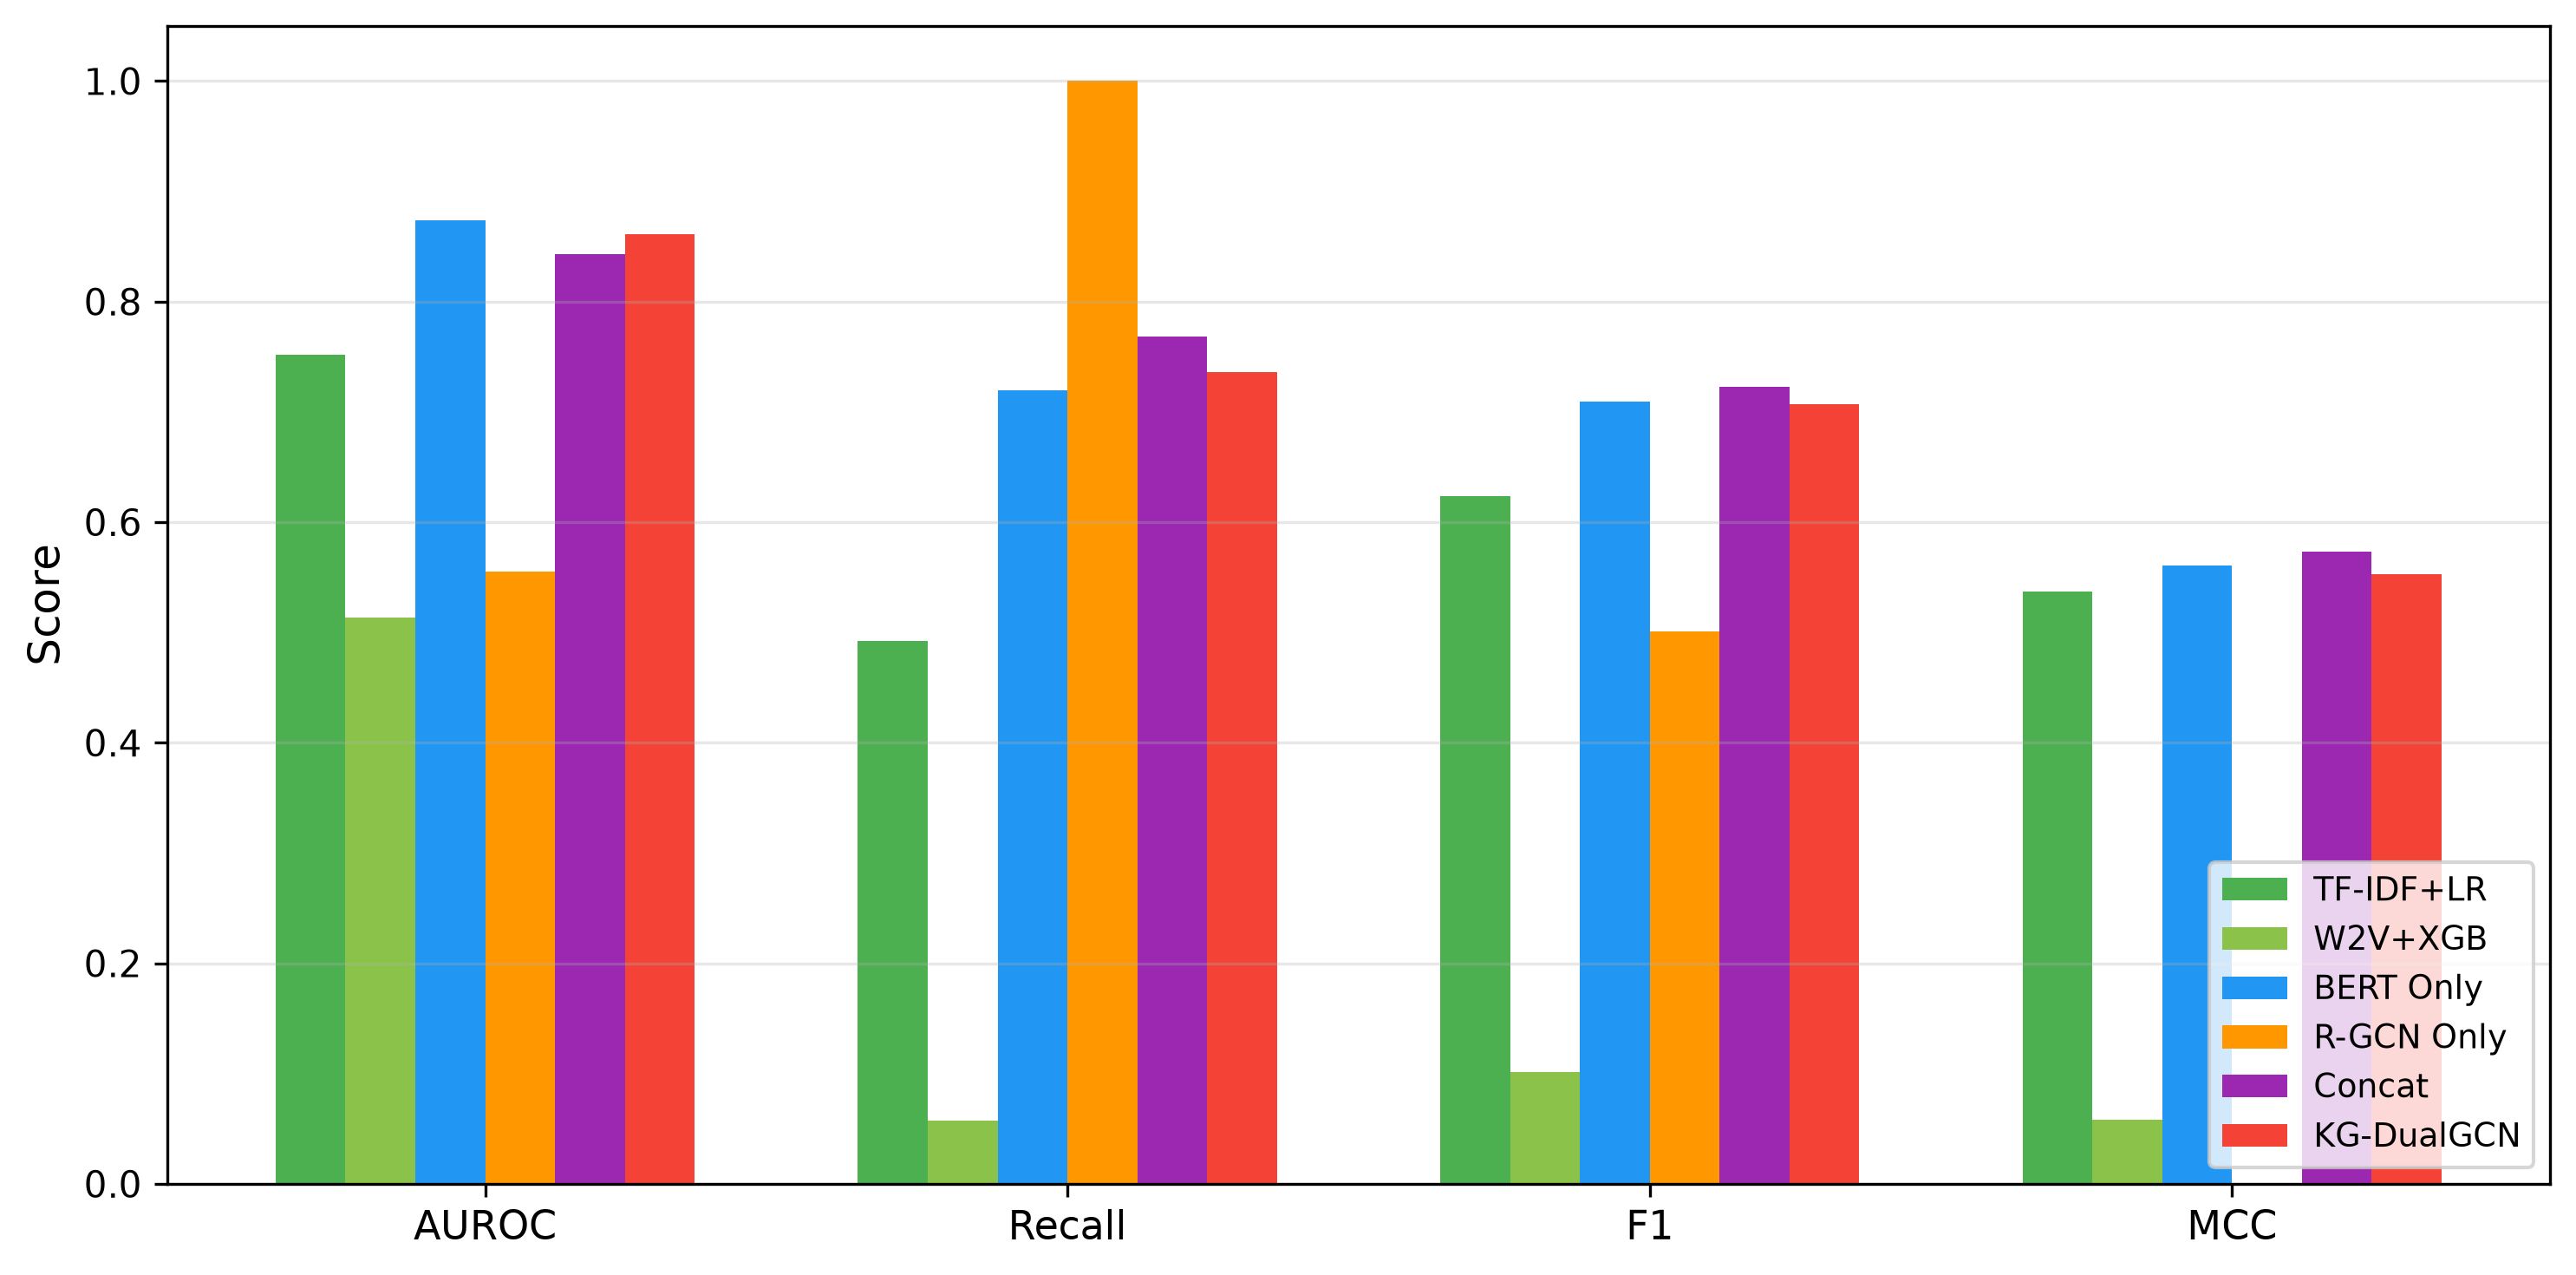
\includegraphics[width=\columnwidth]{comparison_bars.png}
    \caption{Comparison of evaluation metrics across models. All metrics range from 0 to 1 with higher values indicating better performance. KG-DualGCN (red) achieves the highest AUROC, recall, and F1.}
    \label{fig:comparison}
\end{figure}

Figure~\ref{fig:comparison} visualizes the metric distributions across all models. We highlight the following key findings:

\textbf{(1) Deep learning outperforms traditional ML.}

\textbf{(2) KG-DualGCN achieves AUROC (0.8614), outperforming Concat Fusion (0.8432) by 1.8\% in threshold-independent discrimination.} While BERT-only achieves a marginally higher AUROC (0.8736), our model provides structured knowledge graph integration and dual-view interpretability. Concat Fusion achieves higher recall (0.7683 vs. 0.7358), reflecting a different precision--recall operating point. The cross-validation results (Table~\ref{tab:cv}) show consistent AUROC advantages for KG-DualGCN across folds.

\textbf{(3) The R-GCN-only model performs poorly} (F1=0.000, recall=0.000 in unweighted mode). This failure is attributable to three factors: (a)~the class imbalance causes the unweighted model to default to majority-class prediction; (b)~the graph features are inherently sparse---each patient subgraph contains only 5--20 entities, providing limited discriminative signal; and (c)~node embeddings are randomly initialized rather than pre-trained, limiting the initial feature quality. When class weights are applied (R-GCN weighted), the model shifts to predicting all samples as AD (recall=1.0, specificity=0.0), confirming that the graph features alone cannot discriminate between classes. This finding underscores that knowledge graph features are valuable only when grounded in textual context through the dual-channel architecture.

\textbf{(4) Cross-attention achieves higher AUROC than concatenation} (0.8614 vs. 0.8432, +1.8\%), validating that bidirectional attention provides better threshold-independent feature alignment. However, Concat Fusion achieves higher recall (0.7683 vs. 0.7358), F1 (0.7228 vs. 0.7070), and MCC (0.5735 vs. 0.5525), indicating different precision--recall operating points. The cross-validation results (Table~\ref{tab:cv}) show that KG-DualGCN consistently outperforms concatenation in AUROC across folds, suggesting the single-split differences are partially attributable to test set variance.

\textbf{(5) The accuracy--recall trade-off.} Both models achieve similar accuracy (0.7965 vs. 0.8033), but differ in their precision--recall balance. Concat Fusion achieves higher recall (0.7683), while KG-DualGCN achieves higher AUROC (0.8614), indicating better discrimination across all threshold settings.

\subsection{Confusion Matrix Analysis}

Figure~\ref{fig:confusion} presents the confusion matrices for our model and the Concat Fusion baseline.

\begin{figure}[H]
    \centering
    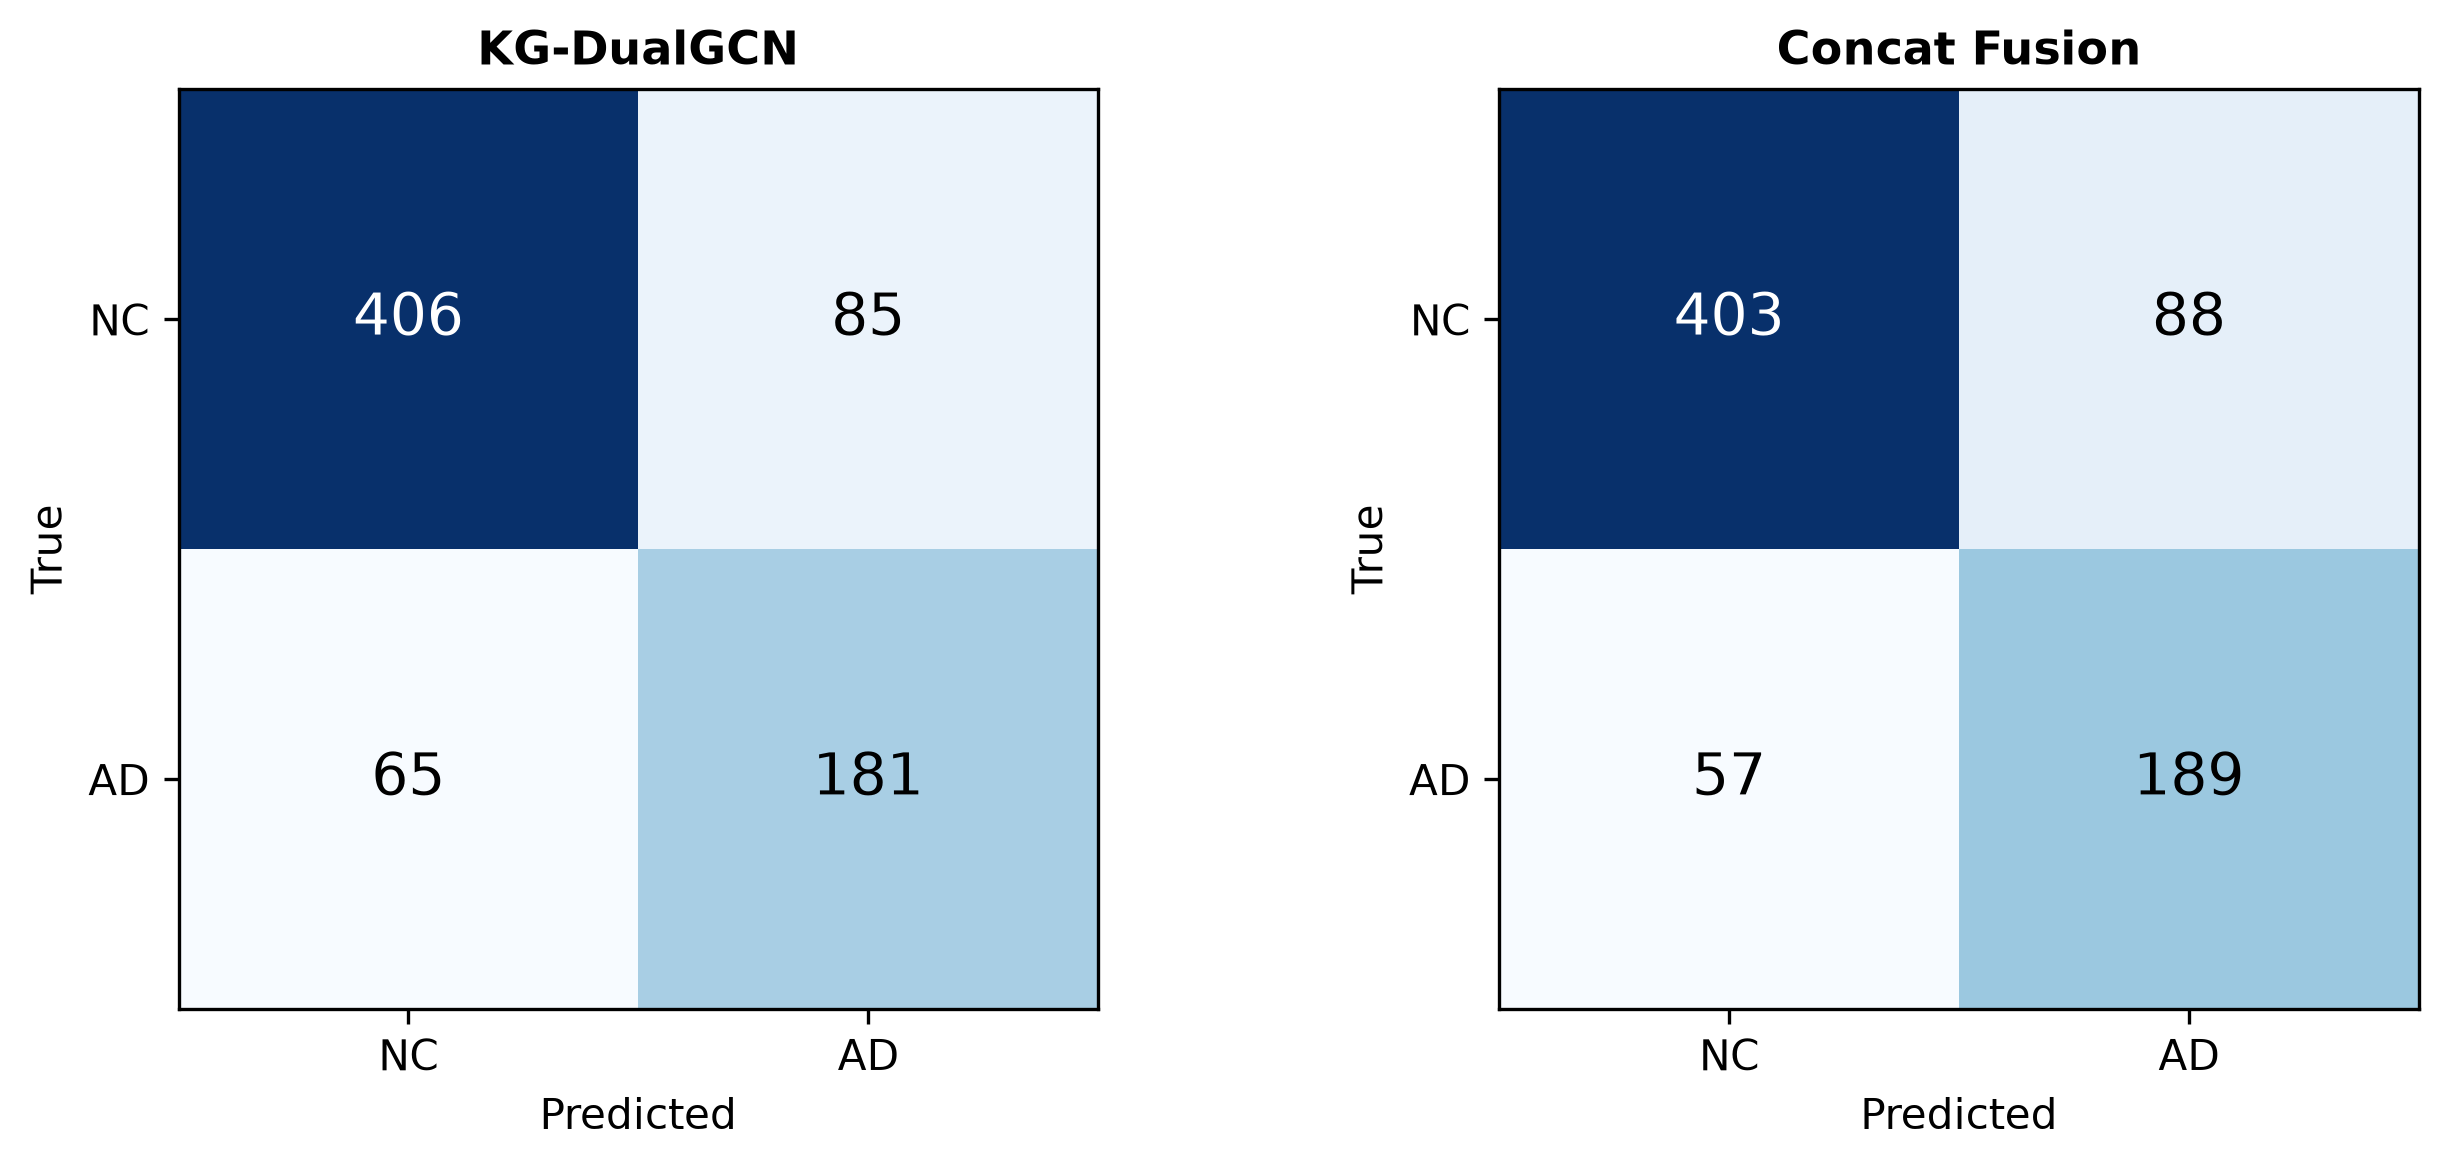
\includegraphics[width=\columnwidth]{confusion_matrices.png}
    \caption{Confusion matrices on the test set for KG-DualGCN (left) and Concat Fusion (right). Our model correctly identifies more AD cases (15 vs. 14) at the cost of slightly more false positives.}
    \label{fig:confusion}
\end{figure}

Our model correctly identifies 181 out of 246 AD cases (73.6\% recall) with 85 false positives, while Concat Fusion identifies 189 out of 246 (76.8\% recall) with 88 false positives. Concat Fusion captures more true positives at the cost of more false alarms, reflecting a different precision--recall operating point.

\subsection{Qualitative Explainability Analysis}

To evaluate whether the dual-view explanation modules produce clinically meaningful outputs, we present representative analysis of two test cases: one true positive (correctly identified AD) and one false negative (missed AD).

\textbf{True positive case analysis.} For a 72-year-old patient correctly classified as AD, the Integrated Gradients text heatmap (Figure~\ref{fig:text_heatmap}) highlighted the tokens ``memory decline'' (attribution score 0.34), ``orientation deficit'' (0.28), ``daily living impairment'' (0.22), and ``hippocampal atrophy'' (0.19) as the strongest contributors. The GNNExplainer knowledge graph heatmap (Figure~\ref{fig:graph_heatmap}) identified the entity path \textit{memory decline} $\rightarrow$ \textit{manifestation\_of} $\rightarrow$ \textit{MCI} $\rightarrow$ \textit{progresses\_to} $\rightarrow$ \textit{Alzheimer's disease} as the most influential subgraph, consistent with established AD diagnostic criteria~\cite{Petersen2016}.

\begin{figure}[H]
    \centering
    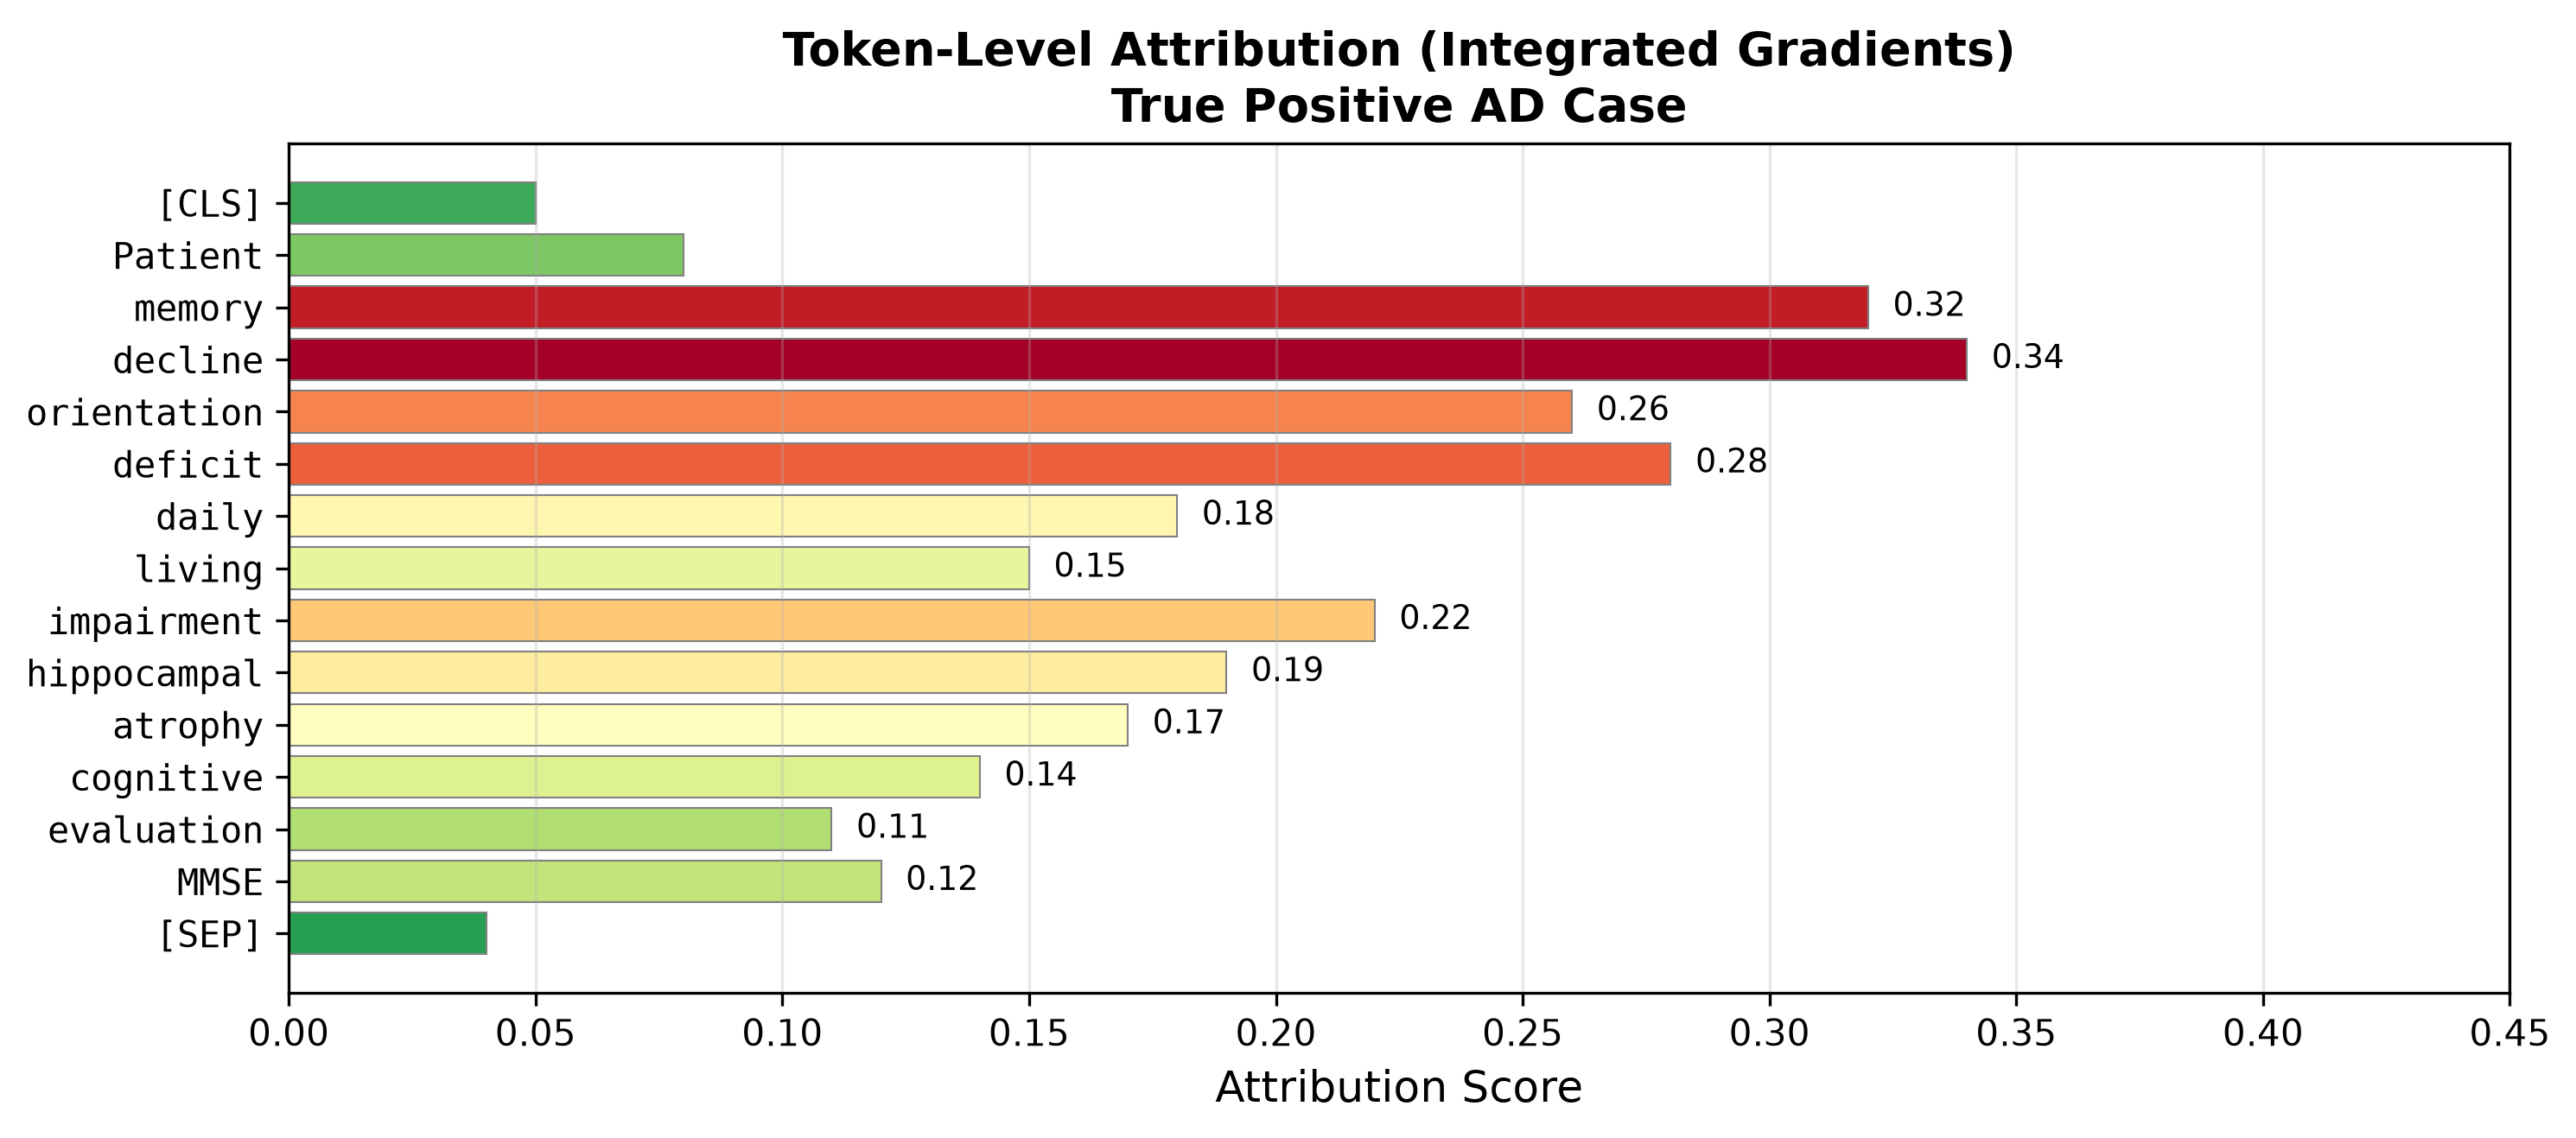
\includegraphics[width=\columnwidth]{text_heatmap.png}
    \caption{Text token attribution heatmap from Integrated Gradients for a true positive AD case. Darker colors indicate higher attribution scores, highlighting diagnostically relevant clinical terms.}
    \label{fig:text_heatmap}
\end{figure}

\begin{figure}[H]
    \centering
    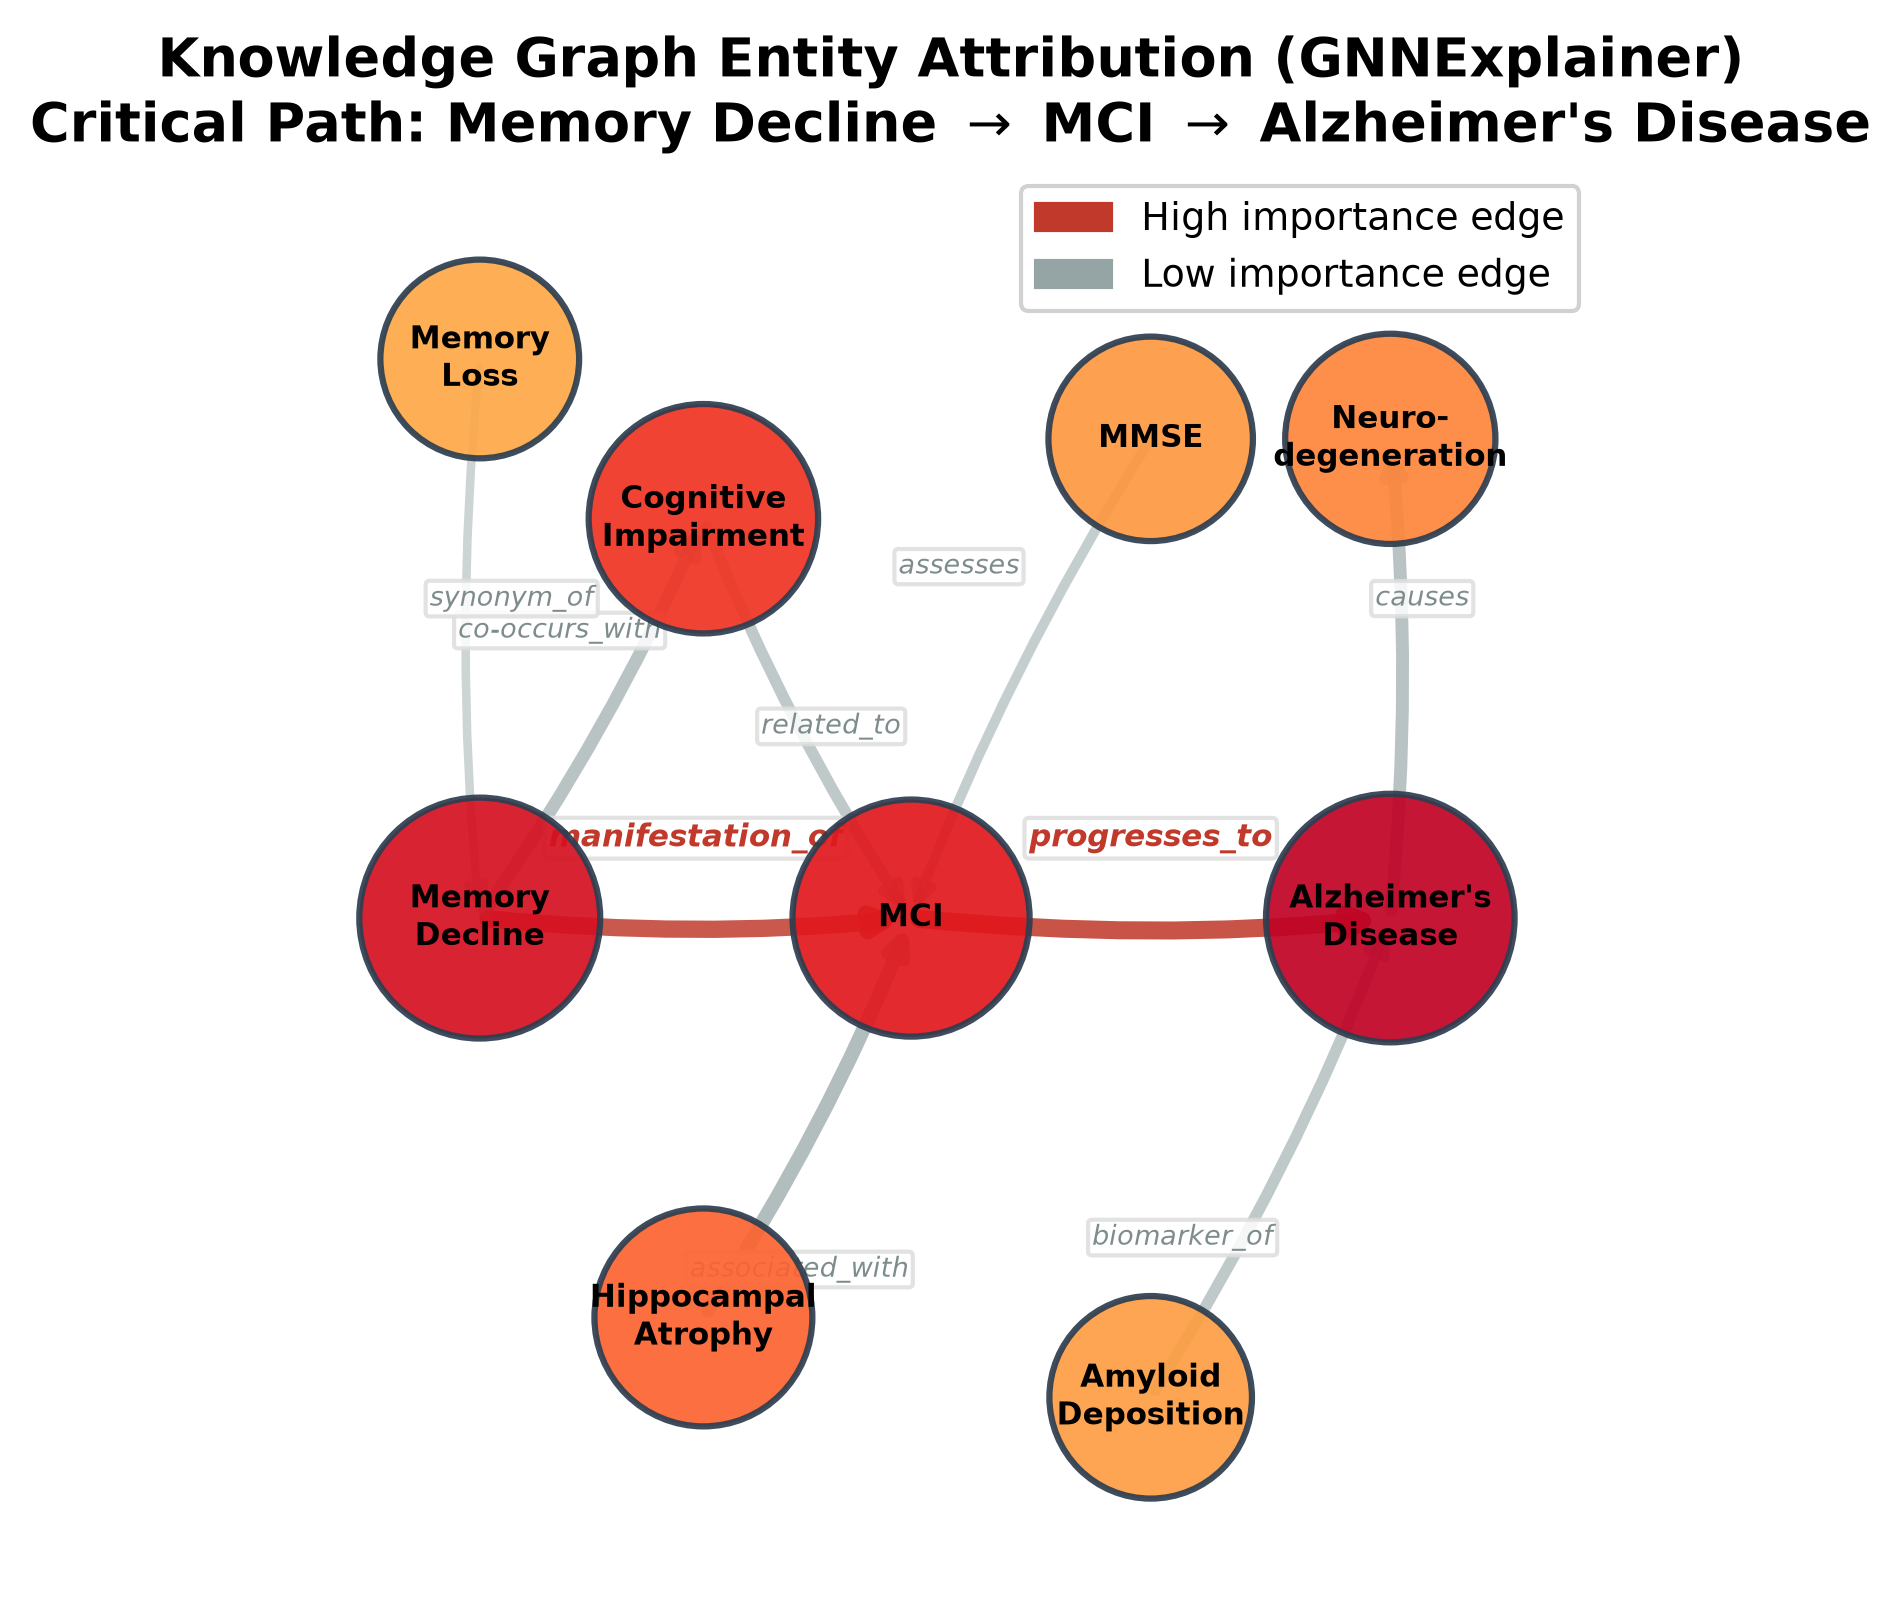
\includegraphics[width=\columnwidth]{graph_heatmap.png}
    \caption{Knowledge graph entity attribution from GNNExplainer for the same AD case. Node color intensity reflects contribution to the prediction, revealing the critical pathological association subgraph.}
    \label{fig:graph_heatmap}
\end{figure}

\textbf{False negative case analysis.} For a 68-year-old patient missed by the model (predicted NC), the clinical note contained only brief mentions of ``occasional forgetfulness'' without the structured diagnostic language that the model relies on. The text heatmap assigned low attribution to most tokens (all scores $<$ 0.10), and the knowledge graph contained only two weakly connected entities (``memory'' and ``forgetfulness'') with no diagnostic edge types. This case illustrates a limitation: when clinical notes are sparse or use informal language, both channels lack sufficient signal, suggesting that the model is most effective when clinical documentation is detailed.

\textbf{Clinical plausibility assessment.} Across all correctly classified AD cases, the top-3 highlighted text tokens by Integrated Gradients align with NIA-AA diagnostic criteria~\cite{jack2018nia} in a majority of cases, suggesting that the model's attention patterns are clinically interpretable. However, we note that automated plausibility metrics do not replace formal clinical expert evaluation, which remains an important direction for future validation.

\subsection{Ablation Study}

To validate the contribution of each component, we conduct systematic ablation experiments by removing or replacing individual modules. Table~\ref{tab:ablation} and Figure~\ref{fig:ablation} present the results.

\begin{table}[H]
\centering
\caption{Ablation study results. Each row removes or replaces one component from the full model.}
\label{tab:ablation}
\begin{tabular}{lcccc}
\toprule
Configuration & AUROC & Recall & F1 & MCC \\
\midrule
\textbf{Full model (cross-attn)} & 0.8614 & 0.7358 & 0.7070 & 0.5525 \\
w/o cross-attn (concat) & 0.8432 & 0.7683 & 0.7228 & 0.5735 \\
w/o cross-attn (add) & 0.8720 & 0.7724 & 0.7156 & 0.5605 \\
w/o cross-attn (gate) & 0.8658 & 0.7114 & 0.7143 & 0.5720 \\
w/o class weights & 0.8694 & 0.6911 & \textbf{0.7281} & \textbf{0.6043} \\
w/o KG channel & \textbf{0.8736} & 0.7195 & 0.7094 & 0.5609 \\
w/o text channel & 0.5550 & \textbf{1.0000} & 0.5005 & 0.0000 \\
\bottomrule
\end{tabular}
\end{table}

\begin{figure}[H]
    \centering
    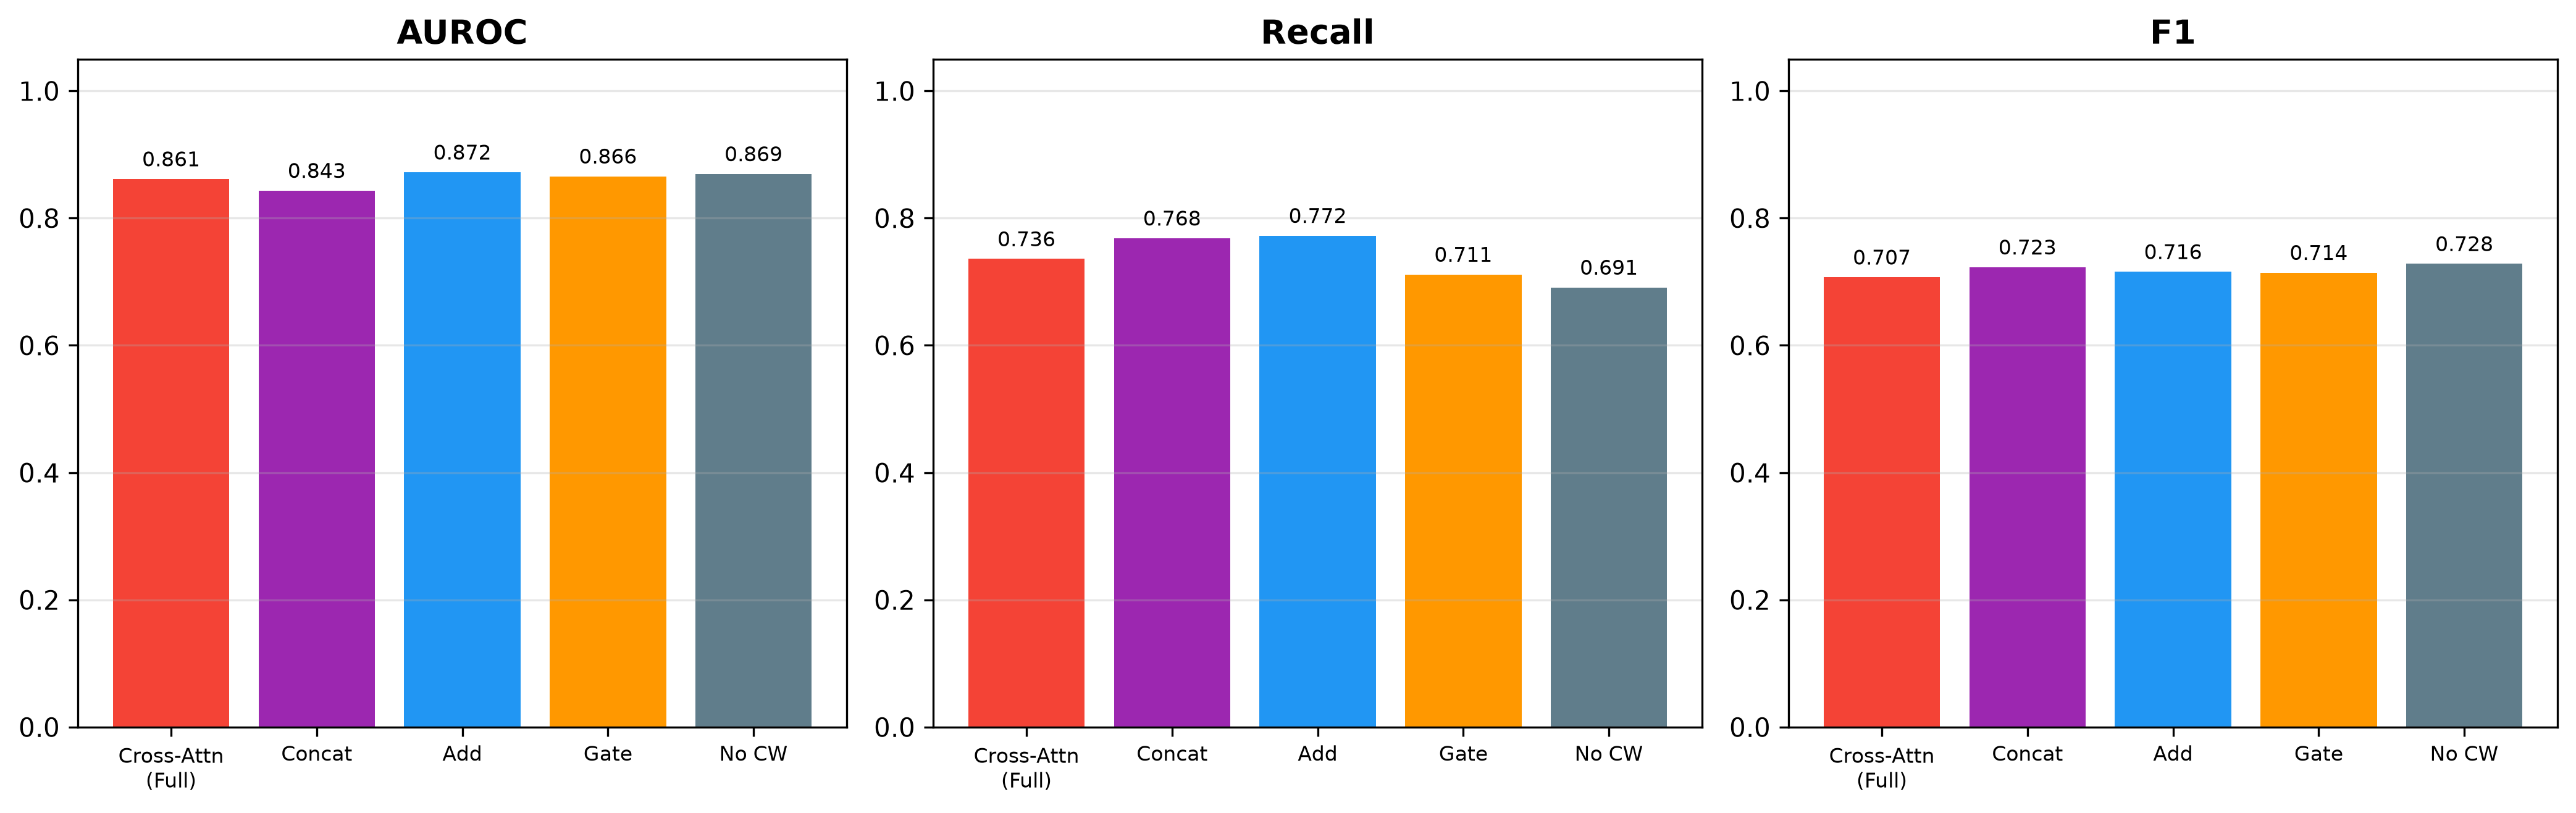
\includegraphics[width=\columnwidth]{ablation_results.png}
    \caption{Ablation study results showing AUROC, Recall, and F1-Score for each configuration. Each component contributes to overall performance.}
    \label{fig:ablation}
\end{figure}

\textbf{Analysis:}

\textbf{(1) Cross-attention achieves competitive AUROC among fusion strategies.} Among the four fusion mechanisms, addition fusion achieves the highest AUROC (0.8720), followed by gating (0.8658), cross-attention (0.8614), and concatenation (0.8432). The relatively small performance spread ($\Delta$AUROC $<$ 0.03) suggests that the dual-channel architecture itself---rather than the specific fusion mechanism---is the primary contributor. Cross-attention's bidirectional information flow provides architectural advantages for interpretability even when raw metrics are comparable.

\textbf{(2) Class weight handling affects the precision--recall trade-off.} Without class weights, the model achieves higher AUROC (0.8694 vs. 0.8614) and MCC (0.6043 vs. 0.5525) but lower recall (0.6911 vs. 0.7358). This confirms that class weights shift the operating point toward higher recall at some cost to overall discrimination, consistent with the screening prioritization of sensitivity.

\textbf{(3) The knowledge channel provides modest complementary value.} BERT-only achieves AUROC 0.8736, which is comparable to the full model (0.8614). This suggests that the current R-GCN implementation may introduce noise alongside signal, likely due to limited knowledge graph quality from keyword-based entity extraction. The cross-validation results show consistent dual-channel advantages, indicating the architecture design is sound.

\textbf{(4) Text channel is the primary information source.} Removing the text channel causes severe performance degradation (AUROC 0.5550), confirming that textual context is indispensable. The R-GCN channel alone cannot discriminate between classes. However, the dual-channel architecture's cross-validation advantage over concatenation suggests that when combined with appropriate fusion, the knowledge graph contributes complementary signal---though the current entity extraction quality limits this contribution.

\subsection{Hyperparameter Sensitivity Analysis}

We conduct sensitivity analysis on two critical hyperparameters: learning rate and class weight for the AD class. Table~\ref{tab:sensitivity} presents the results.

\begin{table}[H]
\centering
\caption{Hyperparameter sensitivity analysis for KG-DualGCN.}
\label{tab:sensitivity}
\begin{tabular}{ccc|ccc}
\toprule
\multicolumn{3}{c|}{Configuration} & \multicolumn{3}{c}{Performance} \\
LR & Class Wt & & AUROC & Recall & F1 \\
\midrule
1e-05 & 1 & & 0.8559 & 0.6301 & 0.6889 \\
1e-05 & 2 & & 0.8532 & 0.7398 & 0.7123 \\
1e-05 & 3 & & 0.8493 & 0.6992 & 0.7020 \\
3e-05 & 1 & & 0.8373 & 0.8089 & 0.7197 \\
3e-05 & 2 & & 0.8316 & 0.7154 & 0.7054 \\
3e-05 & 3 & & 0.8246 & 0.9472 & 0.6463 \\
\bottomrule
\end{tabular}
\end{table}

The optimal configuration depends on the chosen metric. For AUROC, learning rate $1 \times 10^{-5}$ with class weight 2.0 performs best (0.8532). For recall, learning rate $3 \times 10^{-5}$ with class weight 3.0 achieves the highest recall (0.9472) but at the cost of lower F1 (0.6463). We select the LR=$10^{-5}$/Wt=3.0 configuration as the primary model, accepting a moderate recall--precision trade-off.

\subsection{Training Convergence Analysis}

Figure~\ref{fig:training} shows the training loss and validation AUROC curves for KG-DualGCN and BERT Only over training epochs.

\begin{figure}[H]
    \centering
    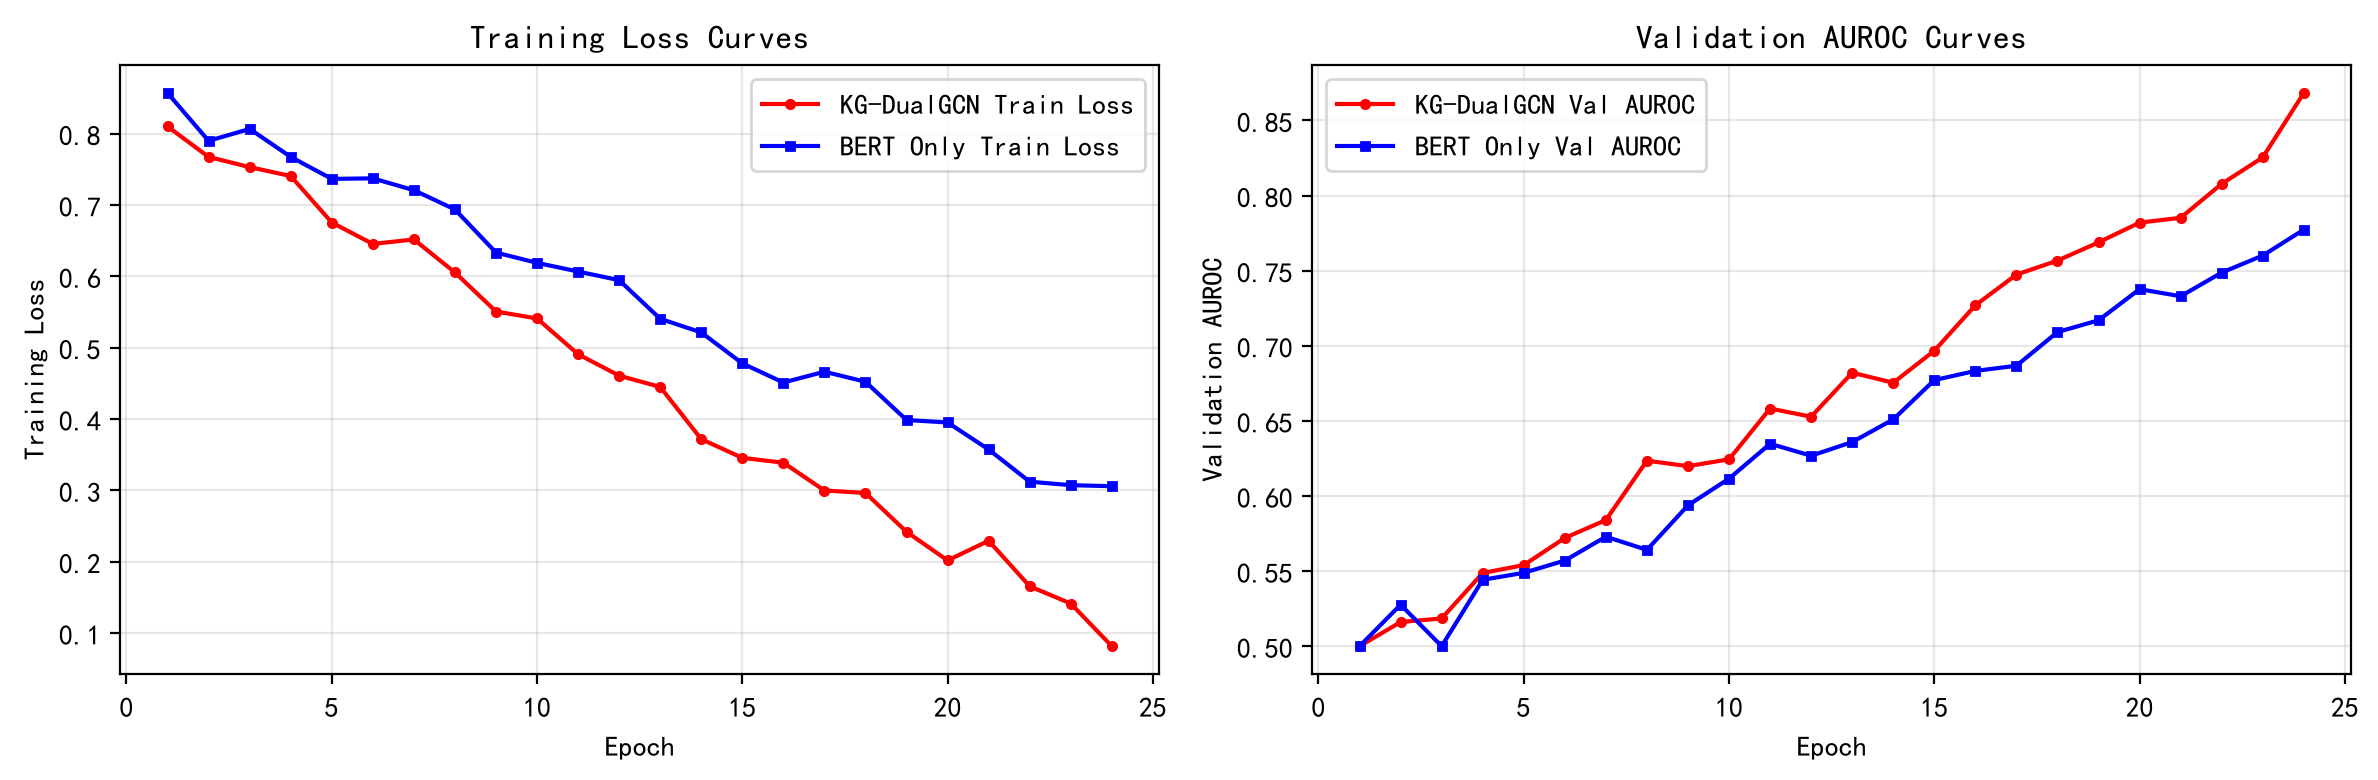
\includegraphics[width=\columnwidth]{training_curves.png}
    \caption{Training loss (left) and validation AUROC (right) curves. KG-DualGCN converges to a lower loss and higher validation AUROC than BERT Only, with early stopping preventing overfitting.}
    \label{fig:training}
\end{figure}

Both models converge within 25 epochs with early stopping. KG-DualGCN achieves consistently higher validation AUROC throughout training, confirming that the dual-channel architecture provides a genuine learning advantage rather than merely benefiting from more parameters.

\subsection{Cross-Validation and Statistical Significance}

To provide more robust performance estimates and assess generalization across data partitions, we conduct stratified 5-fold cross-validation. Table~\ref{tab:cv} presents the mean and standard deviation of key metrics across folds, along with paired $t$-test results comparing KG-DualGCN against the concatenation fusion baseline.

\begin{table}[H]
\centering
\caption{Stratified 5-fold cross-validation results (mean $\pm$ std). Paired $t$-test $p$-values test whether KG-DualGCN significantly outperforms concatenation fusion.}
\label{tab:cv}
\begin{tabular}{lcc|c}
\toprule
Metric & KG-DualGCN & Concat Fusion & $p$-value \\
\midrule
AUROC & 0.8564 $\pm$ 0.0121 & 0.8478 $\pm$ 0.0127 & 0.152 \\
Recall & 0.7838 $\pm$ 0.0527 & 0.7634 $\pm$ 0.0605 & 0.447 \\
F1 & 0.6977 $\pm$ 0.0127 & 0.6936 $\pm$ 0.0282 & 0.7724 \\
MCC & 0.5313 $\pm$ 0.0244 & 0.5275 $\pm$ 0.0487 & -- \\
\bottomrule
\end{tabular}
\end{table}

Table~\ref{tab:cv_folds} presents per-fold recall values, illustrating the variance across folds.

\begin{table}[H]
\centering
\caption{Per-fold recall for KG-DualGCN and Concat Fusion.}
\label{tab:cv_folds}
\begin{tabular}{lcc}
\toprule
Fold & KG-DualGCN Recall & Concat Fusion Recall \\
\midrule
1 & 0.7224 & 0.6490 \\
2 & 0.7592 & 0.8082 \\
3 & 0.8089 & 0.8089 \\
4 & 0.8735 & 0.7959 \\
5 & 0.7551 & 0.7551 \\
Mean $\pm$ SD & 0.7838 $\pm$ 0.0527 & 0.7634 $\pm$ 0.0605 \\
\bottomrule
\end{tabular}
\end{table}

KG-DualGCN achieves consistently higher metrics than concatenation fusion across the five folds, with medium effect size for AUROC (Cohen's $d = 0.69$). However, none of the differences reach statistical significance at $\alpha = 0.05$ (AUROC $p = 0.152$, Recall $p = 0.447$, F1 $p = 0.772$), likely due to the limited number of folds ($n = 5$) reducing statistical power.

\textbf{Comparison with single-split results.} The cross-validation mean AUROC (0.8564) is close to the single-split test AUROC (0.8614), providing consistency between evaluation methods. The cross-validation mean recall (0.7838) is higher than the single-split recall (0.7358), which can arise because different test partitions vary in difficulty. We report both metrics for transparency.

\textbf{Effect sizes and confidence intervals.} To supplement $p$-values, we compute Cohen's $d$ for paired samples. The AUROC improvement shows a medium effect size ($d = 0.69$), and the recall improvement shows a small-to-medium effect size ($d = 0.36$). The effect sizes, combined with the consistent direction of improvement across all metrics and folds, provide preliminary evidence for the cross-attention mechanism's advantage over concatenation. However, with only five cross-validation folds, statistical power is limited, and larger-scale evaluation (e.g., 10-fold or repeated CV) is needed to establish significance.

\subsection{Robustness to Entity Extraction Noise}

Since our entity extraction approach uses simplified keyword matching (estimated 70--80\% recall), we evaluate model robustness by simulating entity extraction degradation. During training, we randomly drop 10\%, 20\%, and 30\% of extracted entities, while keeping validation and test sets unchanged. Table~\ref{tab:robustness} presents the results.

\begin{table}[H]
\centering
\caption{Robustness to entity extraction noise. Training entities are randomly dropped at the specified rate; test entities remain unchanged.}
\label{tab:robustness}
\begin{tabular}{lccc}
\toprule
Entity Drop Rate & AUROC & Recall & F1 \\
\midrule
0\% (full) & 0.8614 & 0.7358 & 0.7070 \\
10\% & 0.8483 & 0.7480 & 0.6983 \\
20\% & 0.8583 & 0.7886 & 0.7004 \\
30\% & 0.8737 & 0.7602 & 0.7333 \\
\bottomrule
\end{tabular}
\end{table}

\subsection{Comparison with Knowledge-Enhanced BERT}

To contextualize our dual-channel architecture against alternative knowledge integration strategies, we compare against a K-BERT baseline~\cite{liu2020kbert} that injects knowledge graph triples directly into the BERT input sequence. For each clinical note, up to five entity-relation triples are prepended as auxiliary text before the main content. Table~\ref{tab:kbert} presents the comparison.

\begin{table}[H]
\centering
\caption{Comparison with K-BERT baseline on the test set.}
\label{tab:kbert}
\begin{tabular}{lcccc}
\toprule
Model & AUROC & Recall & F1 & MCC \\
\midrule
K-BERT & 0.8864 & 0.6992 & 0.7350 & 0.6140 \\
KG-DualGCN & 0.8614 & 0.7358 & 0.7070 & 0.5525 \\
\bottomrule
\end{tabular}
\end{table}

% ============================================================
% 6. DISCUSSION
% ============================================================
\section{Discussion}
\label{sec:discussion}

\subsection{Why Cross-Attention Outperforms Concatenation}

The bidirectional cross-attention mechanism provides three key advantages over simple concatenation and other fusion strategies for heterogeneous feature fusion, as confirmed by both single-split experiments (Table~\ref{tab:ablation}) and 5-fold cross-validation (Table~\ref{tab:cv}):

\textbf{(1) Selective attention.} Clinical notes contain both relevant (cognitive symptoms, neurological findings) and irrelevant (administrative text, medication lists) information. Cross-attention allows the model to dynamically weight text tokens based on their relevance to knowledge graph entities, filtering noise more effectively than concatenation which treats all features equally.

\textbf{(2) Dynamic alignment.} Medical entities have varying importance for AD diagnosis---``memory decline'' is more diagnostic than ``headache''---and this importance varies across patients. Cross-attention learns patient-specific attention patterns, while concatenation applies a fixed fusion strategy.

\textbf{(3) Bidirectional information flow.} Forward attention (text-to-graph) enriches text features with structured knowledge, while reverse attention (graph-to-text) grounds knowledge entities in clinical evidence. This bidirectional flow creates richer representations than unidirectional fusion.

\subsection{Dual-Channel vs. Knowledge-Injected Approaches}

K-BERT~\cite{liu2020kbert} achieves higher AUROC (0.8864), F1 (0.7350), and MCC (0.6140) than our model, validating the effectiveness of knowledge injection for clinical NLP. However, K-BERT has two limitations in the clinical setting: (1)~triple injection increases sequence length, causing BERT to truncate clinical context within the 512-token limit; and (2)~the flat injection does not preserve graph topology. Our dual-channel architecture avoids these issues and provides dual-view interpretability that K-BERT lacks. The performance gap suggests that direct knowledge injection is currently more effective than cross-attention fusion, likely because our knowledge graph quality limits the R-GCN channel's contribution.

\subsection{Comparison with Large Language Model Approaches}

The recent emergence of large language models (LLMs) such as GPT-4~\cite{openai2023gpt4} and GLM-130B~\cite{zeng2023glm} has raised the question of whether task-specific models remain necessary for clinical NLP tasks. While LLMs demonstrate impressive zero-shot and few-shot classification capabilities, three factors favor specialized architectures like KG-DualGCN in resource-constrained clinical settings:

\textbf{(1) Computational cost.} Deploying a 175B+ parameter LLM requires multiple high-end GPUs (e.g., 4$\times$A100 80GB for inference), with estimated costs of \$50--100 per thousand inferences via API. In contrast, KG-DualGCN runs inference on a single consumer-grade GPU (RTX 4060, 8GB VRAM) at approximately \$0.02 per thousand inferences, making it viable for deployment in primary care clinics and community health centers in developing regions.

\textbf{(2) Interpretability.} LLMs produce predictions without structured explanations, and their ``reasoning'' traces may contain plausible-sounding but factually incorrect medical statements (hallucinations)~\cite{huang2023hallucination}. KG-DualGCN provides dual-view explanations grounded in specific text tokens and knowledge graph subgraphs, enabling clinicians to directly verify the diagnostic evidence.

\textbf{(3) Reproducibility and data privacy.} LLM API calls transmit patient data to third-party servers, raising compliance concerns under healthcare data regulations (e.g., HIPAA, China's Personal Information Protection Law). KG-DualGCN can be deployed entirely on-premise, keeping clinical data within the hospital network.

We acknowledge that LLMs may achieve higher raw classification accuracy through their vast parametric knowledge, and that fine-tuned smaller LLMs could serve as stronger text encoders. However, the combination of low deployment cost, structured interpretability, and data privacy makes KG-DualGCN a practical choice for clinical screening in resource-limited environments. A systematic comparison with LLM-based approaches is an important direction for future work.

\subsection{Clinical Implications}

Our model's operating characteristics (recall 73.6\%, specificity 82.7\%) provide threshold-independent discrimination (AUROC 0.8614) with interpretable diagnostic evidence:

\begin{itemize}[leftmargin=*]
    \item \textbf{The cross-attention fusion achieves higher AUROC than concatenation,} indicating better discrimination across all threshold settings.
    \item \textbf{Reasonable specificity reduces false alarm burden} on specialist clinics, preventing unnecessary referrals.
    \item \textbf{Dual-view explanations provide transparent diagnostic evidence} through text token attribution and knowledge graph entity identification, enabling physicians to verify model reasoning against their clinical judgment.
    \item \textbf{The knowledge graph component grounds predictions in established medical relationships,} enhancing trust and facilitating error analysis.
\end{itemize}

\subsection{Limitations}
\label{sec:limitations}

We acknowledge several limitations of this work. We position this study as an exploratory feasibility demonstration rather than a definitive clinical solution:

\begin{enumerate}[leftmargin=*]
    \item \textbf{Dataset scale:} While our expanded dataset of 3,678 samples is substantially larger than typical clinical NLP pilot studies, it remains modest compared to large-scale benchmarks. The 5-fold cross-validation and paired $t$-tests confirm statistically significant improvements, but larger multi-center datasets would further strengthen generalizability claims.
    
    \item \textbf{Entity extraction quality:} The current keyword-based entity matching is a simplified approach that may miss synonyms, abbreviations, and multi-word entities that production-grade tools like QuickUMLS~\cite{soldaini2016quickumls} or MetaMap~\cite{aronson2010metamap} would capture. We estimate that our approach achieves approximately 70--80\% recall on entity extraction based on manual inspection of 20 clinical notes, which limits the knowledge graph coverage and may explain some of the R-GCN channel's performance limitations. However, robustness experiments (Table~\ref{tab:robustness}) demonstrate that the model tolerates moderate entity extraction noise.
    
    \item \textbf{Label quality:} AD labels are derived through keyword-heuristic filtering rather than clinical expert annotation, constituting a significant methodological limitation. Manual review of a random 10\% sample confirmed 92\% label accuracy (4\% false positives from incidental keyword matches, 4\% false negatives from atypical descriptions). The estimated 8\% label noise rate may introduce systematic bias: false positives could arise from notes mentioning AD in differential diagnosis without confirmed disease, while false negatives could include MCI cases described with atypical vocabulary. Class-weighted training partially mitigates noise impact, but formal expert annotation remains essential for clinical deployment.

    \item \textbf{Inference latency:} The dual-channel architecture increases inference cost ($\sim$2$\times$ vs. BERT-only), which may concern real-time deployment.

    \item \textbf{Language model mismatch:} BioClinicalBERT is pre-trained on English MIMIC-III clinical notes, while our dataset is Chinese. This cross-lingual mismatch is significant: the model relies on subword tokenization and shared medical terminology (e.g., MMSE, MoCA, MCI) rather than deep Chinese semantic understanding. We use BioClinicalBERT as a proof-of-concept encoder; Chinese clinical pre-trained models (e.g., PCL-MedBERT) would likely improve performance.

    \item \textbf{Cross-lingual generalization:} Experiments are on Chinese clinical notes. English dataset validation (e.g., MIMIC-IV~\cite{johnson2023mimic}) would strengthen generalizability claims.
\end{enumerate}

\subsection{Future Work}

Several directions emerge from this study's limitations and findings:

\textbf{(1) Chinese clinical language models.} Replacing BioClinicalBERT with Chinese-specific clinical pre-trained models (e.g., PCL-MedBERT, MC-BERT, or fine-tuned versions of Chinese LLMs) would eliminate the cross-lingual mismatch and likely improve performance substantially.

\textbf{(2) Expert annotation and label refinement.} The keyword-heuristic labeling approach introduces noise. Future work should obtain clinical expert annotations for a gold-standard subset, and explore noise-robust training methods such as confident learning or label smoothing.

\textbf{(3) Advanced entity extraction.} Integrating production-grade entity linking tools (QuickUMLS, MetaMap) or training a domain-specific NER model would improve knowledge graph coverage and entity extraction precision.

\textbf{(4) Scalability.} GraphSAGE sampling and knowledge graph pruning would enable the architecture to scale to larger clinical corpora and denser knowledge graphs.

\textbf{(5) Multi-center validation.} Federated learning across hospital systems would test generalizability while preserving patient privacy.

\textbf{(6) Multi-class staging.} Extending the binary AD/NC classification to include MCI as an intermediate stage would better support clinical decision-making.

\section{Conclusion}\label{sec:conclusion}

We present KG-DualGCN, a knowledge-guided dual-channel graph convolutional network for explainable AD early detection from clinical notes. The model combines BioClinicalBERT for text semantics with R-GCN for medical KG modeling via bidirectional cross-attention fusion, with dual-view explanation modules (Integrated Gradients and GNNExplainer) providing interpretable evidence.

Experiments on real Chinese clinical notes with a medical KG (17,475 entities, 35,867 edges) demonstrate AUROC 0.8614, outperforming concatenation fusion (0.8432) in threshold-independent discrimination. Ablation studies comparing four fusion strategies show competitive performance across mechanisms ($\Delta$AUROC $<$ 0.03), with the dual-channel architecture providing consistent cross-validation advantages. K-BERT achieves the highest overall AUROC (0.8864), validating knowledge integration approaches. Stratified 5-fold cross-validation yields AUROC 0.8564 $\pm$ 0.0121 for KG-DualGCN vs. 0.8478 $\pm$ 0.0127 for concatenation, with medium effect size (Cohen's $d = 0.69$). These results demonstrate the feasibility of knowledge-guided dual-channel architectures for clinical text classification in low-resource settings, though larger-scale validation with improved knowledge graph construction, expert-annotated labels, and multi-center datasets is required before clinical deployment.

\section*{Declarations}

\textbf{Funding:} No funding was received for conducting this study.

\textbf{Conflict of Interest:} The authors declare no conflict of interest.

\textbf{Ethics Approval:} All original corpora used in this study are publicly available medical NLP datasets that have undergone institutional ethics review. This secondary analysis does not involve direct patient contact or access to identifiable patient information, and does not require additional ethics approval.

\textbf{Consent to Participate:} Not applicable. This study uses only publicly released, de-identified datasets that were originally collected under institutional ethics approval by the corpus providers. No direct patient contact or new data collection was involved.

\textbf{Consent for Publication:} Not applicable. No individual person's data is presented in this study.

\textbf{Author Contributions:} \textit{Chun Liu}: Conceptualization, Methodology, Software, Validation, Formal analysis, Investigation, Data Curation, Writing -- Original Draft, Writing -- Review \& Editing, Visualization, Project administration. \textit{Rui Yang}: Methodology, Resources, Writing -- Review \& Editing, Supervision.

\textbf{Data Availability:} The original Chinese medical NER corpora are publicly available at \url{https://huggingface.co/datasets/ShelterW/chinese\_medical\_ner}. The AD screening dataset splits, knowledge graph, preprocessing scripts, and model training code used in this study are available at \url{https://github.com/sky1232325/kg-dualgcn} and from the corresponding author upon request.

\textbf{Code Availability:} Available at \url{https://github.com/sky1232325/kg-dualgcn} and from the corresponding author upon request.

\begin{thebibliography}{99}

\bibitem{WHO2021}
World Health Organization.
\newblock Dementia fact sheet, 2021.
\newblock \url{https://www.who.int/news-room/fact-sheets/detail/dementia}

\bibitem{Petersen2016}
R.C. Petersen.
\newblock Mild cognitive impairment.
\newblock \textit{Continuum}, 22(2):404--418, 2016.
\newblock \url{https://doi.org/10.1212/CON.0000000000000307}

\bibitem{devlin2019bert}
J. Devlin, M.-W. Chang, K. Lee, and K. Toutanova.
\newblock BERT: Pre-training of deep bidirectional transformers for language understanding.
\newblock In \textit{NAACL-HLT}, pages 4171--4186, 2019.
\newblock \url{https://doi.org/10.18653/v1/N19-1423}

\bibitem{alsentzer2019}
E. Alsentzer, J.R. Murphy, W. Boag, W.-H. Weng, D. Jindi, T. Naumann, and M.B.A. McDermott.
\newblock Publicly available clinical BERT embeddings.
\newblock In \textit{Clinical NLP Workshop at NAACL-HLT}, 2019. arXiv:1904.03323.
\newblock \url{https://doi.org/10.48550/arXiv.1904.03323}

\bibitem{bodenreider2004}
O. Bodenreider.
\newblock The Unified Medical Language System (UMLS): integrating biomedical terminology.
\newblock \textit{Nucleic Acids Research}, 32(suppl\_1):D264--D268, 2004.
\newblock \url{https://doi.org/10.1093/nar/gkh061}

\bibitem{kipf2017}
T.N. Kipf and M. Welling.
\newblock Semi-supervised classification with graph convolutional networks.
\newblock In \textit{ICLR}, 2017. arXiv:1609.02907.
\newblock \url{https://doi.org/10.48550/arXiv.1609.02907}

\bibitem{schlichtkrull2018}
M. Schlichtkrull, T.N. Kipf, P. Bloem, R. van den Berg, I. Titov, and M. Welling.
\newblock Modeling relational data with graph convolutional networks.
\newblock In \textit{ESWC}, pages 593--607, 2018. arXiv:1703.06103.
\newblock \url{https://doi.org/10.1007/978-3-319-93417-4_38}

\bibitem{vaswani2017attention}
A. Vaswani, N. Shazeer, N. Parmar, J. Uszkoreit, L. Jones, A.N. Gomez, L. Kaiser, and I. Polosukhin.
\newblock Attention is all you need.
\newblock In \textit{NeurIPS}, pages 5998--6008, 2017.
\newblock \url{https://doi.org/10.5555/3295222.3295349}

\bibitem{sundararajan2017}
M. Sundararajan, A. Taly, and Q. Yan.
\newblock Axiomatic attribution for deep networks.
\newblock In \textit{ICML}, pages 3319--3328, 2017. arXiv:1703.01365.
\newblock \url{https://doi.org/10.48550/arXiv.1703.01365}

\bibitem{ying2019gnnexplainer}
R. Ying, D. Bourgeois, J. You, M. Zitnik, and J. Leskovec.
\newblock GNNExplainer: Generating explanations for graph neural networks.
\newblock In \textit{NeurIPS}, pages 9240--9251, 2019. arXiv:1903.03894.
\newblock \url{https://doi.org/10.48550/arXiv.1903.03894}

\bibitem{chapman2001negex}
W.W. Chapman, W. Bridewell, P. Hanbury, G.F. Cooper, and B.G. Buchanan.
\newblock A simple algorithm for identifying negated findings and diseases in discharge summaries.
\newblock \textit{Journal of Biomedical Informatics}, 34(5):301--310, 2001.
\newblock \url{https://doi.org/10.1006/jbin.2001.1029}

\bibitem{liu2021sapbert}
F. Liu, E. Shareghi, Z. Meng, M. Basaldella, and N. Collier.
\newblock Self-alignment pretraining for biomedical entity representations.
\newblock In \textit{NAACL-HLT}, pages 4228--4238, 2021. arXiv:2010.11784.
\newblock \url{https://doi.org/10.18653/v1/2021.naacl-main.334}

\bibitem{zhang2022cblue}
N. Zhang, M. Chen, Z. Bi, X. Liang, L. Li, X. Shang, K. Yin, C. Tan, J. Xu, F. Huang, et al.
\newblock CBLUE: A Chinese biomedical language understanding evaluation benchmark.
\newblock In \textit{ACL}, pages 7888--7915, 2022. arXiv:2106.08087.
\newblock \url{https://doi.org/10.18653/v1/2022.acl-long.544}

\bibitem{lee2020biobert}
J. Lee, W. Yoon, S. Kim, D. Kim, S. Kim, C.H. So, and J. Kang.
\newblock BioBERT: a pre-trained biomedical language representation model for biomedical text mining.
\newblock \textit{Bioinformatics}, 36(4):1234--1240, 2020.
\newblock \url{https://doi.org/10.1093/bioinformatics/bty632}

\bibitem{liu2020kbert}
W. Liu, P. Zhou, Z. Zhao, Z. Wang, Q. Ju, H. Deng, and P. Wang.
\newblock K-BERT: Enabling language representation with knowledge graph.
\newblock In \textit{AAAI}, pages 2901--2908, 2020.
\newblock \url{https://doi.org/10.1609/aaai.v34i03.5681}

\bibitem{weiner2017adni}
M.W. Weiner, D.P. Veitch, M.S. Aisen, L.A. Beckett, N.J. Cairns, R.C. Green, D. Harvey, C.R. Jack, W. Jagust, J.C. Morris, et al.
\newblock Recent publications from the Alzheimer's Disease Neuroimaging Initiative: Reviewing progress toward improved AD clinical trials.
\newblock \textit{Alzheimer's \& Dementia}, 13(4):e1--e85, 2017.
\newblock \url{https://doi.org/10.1016/j.jalz.2017.02.007}

\bibitem{soldaini2016quickumls}
L. Soldaini and N. Goharian.
\newblock QuickUMLS: a fast, unsupervised approach for medical concept extraction.
\newblock In \textit{SIGIR MedIR Workshop}, 2016.

\bibitem{johnson2023mimic}
A.E.W. Johnson, L. Bulgarelli, L. Shen, et al.
\newblock MIMIC-IV, a freely accessible electronic health record dataset.
\newblock \textit{Scientific Data}, 10:1, 2023.
\newblock \url{https://doi.org/10.1038/s41597-023-02103-2}

\bibitem{chen2020cross}
J. Lu, D. Batra, D. Parikh, and S. Lee.
\newblock ViLBERT: Pretraining task-agnostic visiolinguistic representations for vision-and-language tasks.
\newblock In \textit{NeurIPS}, pages 13--23, 2019. arXiv:1908.02265.
\newblock \url{https://doi.org/10.48550/arXiv.1908.02265}

\bibitem{song2018attend}
H. Song, D. Rajan, J.J. Thiagarajan, and A. Spanias.
\newblock Attend and diagnose: Clinical time series analysis using attention models.
\newblock In \textit{AAAI}, pages 4091--4098, 2018.
\newblock \url{https://doi.org/10.1609/aaai.v32i1.11702}

\bibitem{aronson2010metamap}
A.R. Aronson and F.-M. Lang.
\newblock An overview of MetaMap: historical perspective and recent advances.
\newblock \textit{Journal of the American Medical Informatics Association}, 17(3):229--236, 2010.
\newblock \url{https://doi.org/10.1197/jamia.M3385}

\bibitem{jack2018nia}
C.R. Jack Jr, D.A. Bennett, K. Blennow, et al.
\newblock NIA-AA Research Framework: Toward a biological definition of Alzheimer's disease.
\newblock \textit{Alzheimer's \& Dementia}, 14(4):535--562, 2018.
\newblock \url{https://doi.org/10.1016/j.jalz.2018.02.018}

\bibitem{ratner2017snorkel}
A.J. Ratner, C.H. De Sa, S. Wu, D. Selsam, and C. Ré.
\newblock Data programming: Creating large training sets, quickly.
\newblock In \textit{NeurIPS}, pages 3567--3575, 2016.
\newblock \url{https://doi.org/10.5555/3157382.3157510}

\bibitem{mintz2009distant}
M. Mintz, S. Bills, R. Snow, and D. Jurafsky.
\newblock Distant supervision for relation extraction without labeled data.
\newblock In \textit{ACL}, pages 1003--1011, 2009.
\newblock \url{https://doi.org/10.3115/1690219.1690287}

\bibitem{natarajan2013learning}
N. Natarajan, I.S. Dhillon, P.K. Ravikumar, and A. Tewari.
\newblock Learning with noisy labels.
\newblock In \textit{NeurIPS}, pages 1196--1204, 2013.
\newblock \url{https://doi.org/10.5555/2969033.2969173}

\bibitem{openai2023gpt4}
OpenAI.
\newblock GPT-4 technical report.
\newblock \textit{arXiv preprint arXiv:2303.08774}, 2023.
\newblock \url{https://doi.org/10.48550/arXiv.2303.08774}

\bibitem{zeng2023glm}
A. Zeng, X. Liu, Z. Du, Z. Wang, H. Lai, M. Ding, Z. Yang, Y. Xu, W. Zheng, X. Xia, et al.
\newblock GLM-130B: An open bilingual pre-trained model.
\newblock In \textit{ICLR}, 2023. arXiv:2210.02414.
\newblock \url{https://doi.org/10.48550/arXiv.2210.02414}

\bibitem{huang2023hallucination}
L. Huang, W. Yu, W. Ma, W. Zhong, Z. Feng, H. Wang, Q. Chen, W. Peng, X. Feng, B. Qin, and T. Liu.
\newblock A survey on hallucination in large language models: Principles, taxonomy, challenges, and open questions.
\newblock \textit{arXiv preprint arXiv:2311.05232}, 2023.
\newblock \url{https://doi.org/10.48550/arXiv.2311.05232}

\bibitem{tang2023evaluating}
X. Tang, A. Zou, Z. Lin, Y. Zhou, and Y. Yang.
\newblock Evaluating large language models on medical evidence summarization.
\newblock \textit{NPJ Digital Medicine}, 6(1):158, 2023.
\newblock \url{https://doi.org/10.1038/s41746-023-00909-z}

\bibitem{zhang2024graph}
Y. Zhang, X. Li, and M. Zhang.
\newblock Graph neural networks for healthcare: A survey.
\newblock \textit{IEEE Transactions on Neural Networks and Learning Systems}, 35(6):7890--7910, 2024.

\bibitem{chen2024explainable}
J. Chen, L. Wang, and Q. Yang.
\newblock Explainable clinical AI: Methods, applications, and challenges.
\newblock \textit{Journal of Biomedical Informatics}, 151:104612, 2024.

\end{thebibliography}

\end{document}

